\documentclass[lettersize,journal]{IEEEtran}
\usepackage{amsmath,amsfonts}
\usepackage{algorithmic}
\usepackage{array}
\usepackage[caption=false,font=normalsize,labelfont=sf,textfont=sf]{subfig}
\usepackage{textcomp}
\usepackage{stfloats}
\usepackage{url}
\usepackage{verbatim}
\usepackage{graphicx}
\usepackage{array}
\usepackage{amssymb}
\usepackage{cuted}
\usepackage{caption}
\usepackage{multirow} 
\usepackage{makecell}
\usepackage{booktabs}
\usepackage{fontawesome}
\usepackage{pifont}
\usepackage{float}
\usepackage{url}
\usepackage{color}
\usepackage{xcolor}
\usepackage{hyperref}

\hypersetup{colorlinks=true,linkcolor=blue,urlcolor=blue}

\newcommand{\cmark}{\ding{51}}%
\newcommand{\xmark}{\ding{55}}%

 % ts
\usepackage{multirow}
\usepackage{makecell}
\usepackage{booktabs}
\usepackage{tabularx}
\usepackage{amssymb}
\usepackage{siunitx}
\usepackage{enumitem}
 
\hyphenation{op-tical net-works semi-conduc-tor IEEE-Xplore}
\def\BibTeX{{\rm B\kern-.05em{\sc i\kern-.025em b}\kern-.08em
    T\kern-.1667em\lower.7ex\hbox{E}\kern-.125emX}}
\usepackage{balance}
\begin{document}
\title{OmniVTA: Visuo-Tactile World Modeling for Contact-Rich \\ Robotic Manipulation}
\author{
Yuhang Zheng$^{1,2*}$,
Songen Gu$^{3*}$,
Weize Li$^{1}$,
Yupeng Zheng$^{1,4\dagger}$,
Yujie Zang$^{1}$,
Shuai Tian$^{4}$,
Xiang Li$^{1,5}$, \\
Ce Hao$^{6}$,
Chen Gao$^{2,7}$, 
Si Liu$^{7}$, 
Haoran Li$^{4}$,
Yilun Chen$^{1}$,
Shuicheng Yan$^{2\dagger}$,
Wenchao Ding$^{1\dagger}$ \\
\textsuperscript{1}\textbf{TARS Robotics},
\textsuperscript{2}National University of Singapore,
\textsuperscript{3}Fudan University,
\textsuperscript{4}CASIA, \\
\textsuperscript{5}Tsinghua University,
\textsuperscript{6}Zhongguancun Academy,
\textsuperscript{7}Beihang University \\
\textsuperscript{$\dagger$} Corresponding Author,
\textsuperscript{*} Equal Contribution \\
}

\maketitle

\begin{strip}
    \centering
    \vspace{-20mm}
    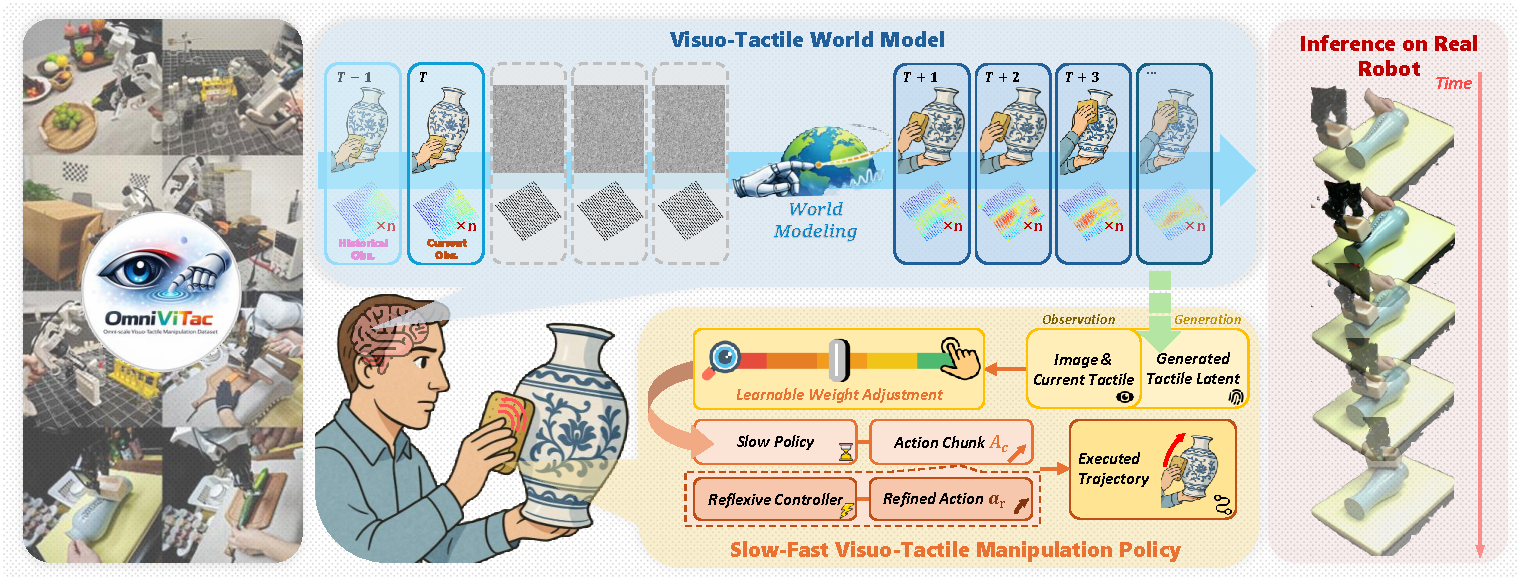
\includegraphics[width=\textwidth]{fig/teaser.pdf}
    \captionof{figure}{\textbf{Overview of the proposed visuo-tactile manipulation system.} (Left) We introduce OmniViTac, a large-scale visuo-tactile-action aligned dataset for contact-rich manipulation. (Center) We propose OmniVTA, a world model-based visuo-tactile-action framework that predicts future contact states. It seamlessly unifies tactile representation learning, predictive multimodal modeling, adaptive fusion, and reflexive tactile control. (Right) Extensive real-world experiments demonstrate that OmniVTA outperforms prior methods, exhibiting strong robustness and generalization.}
    \label{fig:teaser}
\end{strip}

\begin{abstract}
Contact-rich manipulation tasks, such as wiping and assembly, require accurate perception of contact forces, friction changes, and state transitions that cannot be reliably inferred from vision alone. Despite growing interest in visuo-tactile manipulation, progress is constrained by two persistent limitations: existing datasets are small in scale and narrow in task coverage, and current methods treat tactile signals as passive observations rather than using them to model contact dynamics or enable closed-loop control explicitly.
In this paper, we present \textbf{OmniViTac}, a large-scale visuo-tactile-action dataset comprising $21{,}000+$ trajectories across $86$ tasks and $100+$ objects, organized into six physics-grounded interaction patterns. Building on this dataset, we propose \textbf{OmniVTA}, a world-model-based visuo-tactile manipulation framework that integrates four tightly coupled modules: a self-supervised tactile encoder, a two-stream visuo-tactile world model for predicting short-horizon contact evolution, a contact-aware fusion policy for action generation, and a 60Hz reflexive controller that corrects deviations between predicted and observed tactile signals in a closed loop.
Real-robot experiments across all six interaction categories show that OmniVTA outperforms existing methods and generalizes well to unseen objects and geometric configurations, confirming the value of combining predictive contact modeling with high-frequency tactile feedback for contact-rich manipulation. All data, models, and code will be made publicly available on the project website at \url{https://mrsecant.github.io/OmniVTA}.
\end{abstract}

\begin{IEEEkeywords}
Visuo-Tactile Manipulation, Visuo-Tactile World Models, Contact-Rich Manipulation
\end{IEEEkeywords}


\section{Introduction}
Contact-rich manipulation tasks, such as wiping and assembly, are ubiquitous in daily human activities. Their successful execution requires not only precise geometric alignment, but also accurate perception and fine-grained control of contact forces, frictional changes, and subtle transitions in contact state~\cite{zhao2024tac, cui2025vi, zhao2025tacman}. Since such information is difficult to infer reliably from vision alone, recent studies~\cite{bi2025vla, xue2025reactive, chen2025multi} have incorporated tactile sensing into imitation learning frameworks to improve visuomotor policies for contact-rich manipulation.

However, despite the growing adoption of tactile sensing in contact-rich manipulation, the broader visuo-tactile manipulation community still faces substantial limitations in both data and methodology. 
(1) On the data side, existing public visuo-tactile manipulation datasets~\cite{bi2025vla, yu2025demonstrating, bu2025agibot} remain limited in both the scale of fully aligned vision-tactile-action demonstrations and the diversity of contact-rich tasks. In particular, the amount of synchronized visual and high-frequency tactile data is still insufficient for learning generalizable visuo-tactile representations and modeling contact dynamics. In addition, the covered scenarios, tasks, and interaction patterns are narrow, making it difficult to capture the broad spectrum of contact mechanisms required in real-world manipulation.
(2) On the methodology side, existing visuo-tactile manipulation approaches remain limited in both representation and control. In most prior works~\cite{huang20243d, wu2025canonical}, tactile signals are incorporated merely as auxiliary observations to the policy network, primarily for contact-state recognition or compensating for visual occlusion, rather than being used to model the evolution of contact dynamics explicitly. At the control level, these methods typically rely on action chunking to generate short action sequences that are then executed in an open-loop manner. Such a design makes it difficult to react promptly to rapid contact changes, including slippage, misalignment, and external disturbances, which are pervasive in contact-rich manipulation. 

In contrast, humans perform such tasks with remarkable dexterity and robustness. Neuroscience studies~\cite{monzee2003effects, wolpert2001motor, kilteni2017sensorimotor, augurelle2003importance} suggest that this ability relies on tightly coupled multi-modal perception, predictive internal models, and rapid tactile feedback control. This combination of predictive modeling and reflexive correction is still largely missing from current visuo-tactile policies.
 

In this paper, we address these limitations from both the data and methodology perspectives. Concretely, we introduce OmniViTac, a large-scale visuo-tactile-action aligned dataset.
Building on this dataset, we further propose OmniVTA, a world-model-based visuo-tactile manipulation framework.

Specifically, OmniViTac is a large-scale visuo-tactile-action aligned dataset for contact-rich manipulation, comprising $21,879$ trajectories spanning $86$ tasks and $100+$ manipulated objects in diverse real-world scenarios. To capture the broad spectrum of contact-rich behaviors encountered in manipulation, we organize the dataset into six physics-grounded visuo-tactile interaction patterns: wiping, peeling, cutting, grasping, assembly, and in-hand adjustment.
To ensure data fidelity, OmniViTac is collected using a unified cross-embodiment platform and processed through a rigorous pipeline that preserves native sensor frequencies, performs precise temporal synchronization across vision, touch, and action streams, and incorporates automated trimming together with human-in-the-loop verification. Beyond scale and data quality, our analysis further shows that OmniViTac captures structured, pattern-specific contact dynamics and reveals two key properties of tactile signals in manipulation, namely spatial locality and contact-driven dynamics. 
These properties make OmniViTac a strong benchmark for learning visuo-tactile representations, predictive contact models, and robust manipulation policies.

Inspired by human sensorimotor control in contact-rich manipulation, an effective robotic system should possess two key capabilities~\cite{wolpert2001motor}: (1) forming feedforward anticipations of contact evolution through predictive modeling, and (2) exploiting tactile feedback for high-frequency closed-loop correction.

To this end, we propose OmniVTA, a world-model-based visuo-tactile manipulation framework composed of four tightly coupled modules. First, TactileVAE learns compact, low-dimensional tactile representations through spatio-temporal encoding and reconstructs continuous tactile deformation fields with an implicit neural decoder, providing structured tactile features for downstream prediction and policy learning. Second, the Visuo-Tactile World Model adopts a two-stream conditional generative architecture to model the temporal evolution of visual observations and tactile signals, thereby forming short-horizon feedforward predictions of contact dynamics. Third, the Adaptive Visuo-Tactile Fusion Policy leverages a Latent Tactile Differential (LTD) Encoder to capture the relationship between current tactile observations and predicted future tactile features, and adaptively fuses visual and tactile information through a contact-aware gating mechanism for action generation. Finally, the Reflexive Latent Tactile Controller uses predicted and observed tactile features to produce fine-grained corrective actions at 60,Hz, enabling rapid closed-loop correction during manipulation.

Extensive real-robot experiments across six tactile interaction pattern categories validate the effectiveness of OmniVTA from three perspectives. First, OmniVTA achieves state-of-the-art performance on diverse contact-rich manipulation tasks, with strong advantages in object diversity, geometric generalization, and disturbance robustness. The full framework further outperforms its open-loop variant, highlighting the importance of high-frequency tactile feedback for stable contact control. Second, mechanistic analyses show that the policy adaptively reweights vision and touch according to the predicted contact state, and that accurate tactile prediction is crucial for reliable action generation. Third, OmniVTA maintains stable performance under unseen geometric configurations and unseen tools, suggesting that it learns transferable contact-relevant structure and dynamics rather than memorizing task-specific trajectories. Together, these results demonstrate the benefit of predictive visuo-tactile world modeling combined with rapid tactile-feedback-based correction.

The main contributions of this paper are three-fold:
(1) We present OmniViTac, a large-scale visuo-tactile-action aligned dataset for contact-rich manipulation spanning six tactile interaction pattern categories, and reveal two key properties of tactile signals: spatial locality and contact-driven dynamics.
(2) We propose OmniVTA, a world-model-based visuo-tactile manipulation framework that integrates tactile representation learning, predictive visuo-tactile world modeling, contact-aware fusion, and high-frequency closed-loop tactile control.
(3) Extensive real-world experiments show that OmniVTA outperforms state-of-the-art baselines across diverse contact-rich manipulation tasks, with strong robustness to perturbations and effective generalization to novel configurations and objects.
\begin{figure*}[ht]
\centering

\includegraphics[width=0.95\linewidth]{fig/dataset_teaser_0318.png}
\caption{\textbf{{Overview of OmniViTac dataset.}} \textbf{Left:} The Cross-Embodiment Data Collection Platform features UNFactory 7-DoF xArm and the TacUMI manipulation interface, both supporting identical end-effectors and diverse tactile sensors (Xense, GelSight Mini, Tac3D, Daimon). \textbf{Middle:} The dataset covers 6 visuo-tactile manipulation patterns, instantiated across 5 semantic scenarios. \textbf{Top-Right:} A scale comparison demonstrates that OmniViTac (21,879 trajectories) significantly exceeds existing visuo-tactile manipulation datasets in tactile-rich data volume. \textbf{Bottom-Right:} The High-quality Data Pipeline ensures reliability through timestamp alignment, visualization, and human-in-the-loop verification.}
\label{fig:dataset_teaser}
\end{figure*}

\section{Related Works}
\subsection{Tactile Sensing and Tactile Representation Learning}
Robotic fine-grained interaction relies on advances in both tactile hardware and representation learning. Existing tactile sensors span multiple physical principles, including capacitive arrays~\cite{xu2024cushsense,xu2016stretch}, piezoresistive sensors~\cite{stassi2014flexible, sundaram2019learning}, and magnetic sensors~\cite{yan2021soft}. Among them, visuo-tactile sensors such as GelSight~\cite{yuan10high} and DIGIT~\cite{lambeta2020digit} have attracted particular attention because they provide high-resolution and robust measurements. By tracking gel deformation with a camera, they reconstruct fine contact geometry and, with marker dots, estimate force and torque.

With such signals available, the focus has shifted from task-specific features to transferable tactile representations. A major line of work learns from paired vision-tactile data through self-supervision or contrastive learning. Sparsh~\cite{higuera2024sparsh} adopts a masked autoencoder, Anytouch~\cite{feng2025anytouch} uses contrastive learning, and UniT~\cite{xu2025unit} introduces a VQGAN-like architecture~\cite{esser2021taming} for compact latent modeling. More recently, tactile sensing has been integrated into MLLMs to align tactile, visual, and textual representations. Representative examples include Binding touch to everything~\cite{yang2024binding}, Octopi~\cite{yu2024octopi}, and VTV-LLM~\cite{xie2025universal}. Octopi-1.5~\cite{yu2025demonstrating} further adds retrieval augmentation to improve predictions for unseen object-tactile pairs. Our study builds on this trend by examining unified visuo-tactile representation learning across four visuo-tactile sensors: GelSight Mini~\cite{yuan10high}, Tac3D~\cite{zhang2022tac3d}, Xense~\cite{xense}, and Daimon~\cite{daimon}.

\subsection{Visuo-Tactile Robotic Manipulation Policies}
Findings from human motor control highlight the importance of tactile feedback for stable manipulation. Prior studies show that cutaneous feedback is essential for maintaining grip stability~\cite{augurelle2003importance} and that the brain uses a unified internal model to predict tactile feedback for both limbs and tools~\cite{kilteni2017sensorimotor, wolpert2001motor}. These results suggest that tactile sensing is fundamental to contact-rich manipulation, where it complements vision under occlusion and provides direct force-related feedback.

Inspired by these insights, robotic manipulation policies increasingly incorporate non-visual inputs. Early visuo-tactile systems such as See-to-Touch~\cite{guzey2024see} and RoboPack~\cite{ai2024robopack} showed that local tactile observations can resolve ambiguities and support fine-grained control when vision is unreliable. Recent work extends this idea to end-to-end manipulation models, including vision-action models such as 3D-ViTac~\cite{huang20243d} and RDP~\cite{xue2025reactive}, as well as vision-language-action models such as VLA-Touch~\cite{bi2025vla}, Tactile-VLA~\cite{huang2025tactile}, and TA-VLA~\cite{zhang2025ta}. However, effectively fusing tactile and visual signals for high-frequency closed-loop control remains difficult. Existing methods often suffer from weak tactile integration or temporal mismatch. Our framework addresses this problem through deeper visuo-tactile fusion, using local tactile feedback to refine global control for robust contact-rich manipulation.

\subsection{Visuo-tactile Manipulation Datasets and Systems}
Early visuo-tactile datasets~\cite{yang2024binding,fu2024touch,yu2024octopi,feng2025anytouch,xie2025universal,yu2025demonstrating} mainly collected static paired observations by pressing handheld tactile sensors against objects, surfaces, or textures. Although useful for multimodal representation learning, they do not provide action trajectories for manipulation. More recent datasets~\cite{li2022see,fang2023rh20t,wu2025freetacman,bi2025vla,cheng2025omnivtla,xu2025exumi,liu2025mla} mount tactile sensors on robotic grippers and record manipulation through UMI~\cite{chi2024universal}, teleoperation, or kinesthetic teaching. These systems capture synchronized vision, touch, and proprioception, enabling visuo-tactile policy learning for contact-rich tasks. Nevertheless, current datasets remain limited in scale, sensor and platform diversity, and temporal alignment between high-frequency tactile streams and visual observations.

Our work addresses these limitations with a multi-platform visuo-tactile manipulation dataset that offers diverse tasks and fully aligned vision, touch, and action sequences, supporting large-scale world-model training for unified visuo-tactile policy learning.

% \documentclass[lettersize,journal]{IEEEtran}
% \usepackage{amsmath,amsfonts}
% \usepackage{algorithmic}
% \usepackage{array}
% \usepackage[caption=false,font=normalsize,labelfont=sf,textfont=sf]{subfig}
% \usepackage{textcomp}
% \usepackage{stfloats}
% \usepackage{url}
% \usepackage{verbatim}
% \usepackage{graphicx}
% \usepackage{array}  
% \usepackage{multirow} 
% \usepackage{makecell}
% \usepackage{booktabs}
% \usepackage{fontawesome}
% \usepackage{pifont}
% \usepackage{float}
% \usepackage{color}
% \newcommand{\cmark}{\ding{51}}%
% \newcommand{\xmark}{\ding{55}}%

 
% \hyphenation{op-tical net-works semi-conduc-tor IEEE-Xplore}
% \def\BibTeX{{\rm B\kern-.05em{\sc i\kern-.025em b}\kern-.08em
%     T\kern-.1667em\lower.7ex\hbox{E}\kern-.125emX}}
% \usepackage{balance}
% \begin{document}
% \title{Imagine the Touch: Learning Contact-Rich Manipulation Policy via Visuo-Tactile World Model}
% \author{IEEE Publication Technology Department
% \thanks{Manuscript created October, 2020; This work was developed by the IEEE Publication Technology Department. This work is distributed under the \LaTeX \ Project Public License (LPPL) ( http://www.latex-project.org/ ) version 1.3. A copy of the LPPL, version 1.3, is included in the base \LaTeX \ documentation of all distributions of \LaTeX \ released 2003/12/01 or later. The opinions expressed here are entirely that of the author. No warranty is expressed or implied. User assumes all risk.}}

% \markboth{Journal of \LaTeX\ Class Files,~Vol.~18, No.~9, September~2020}%
% {How to Use the IEEEtran \LaTeX \ Templates}

% \maketitle


\section{The OmniViTac Dataset}
% To advance contact-rich manipulation with tactile feedback, we introduce \textbf{OmniViTac}, a comprehensive, omni-scale visuo-tactile-action dataset. It comprises 21,879 trajectories, featuring RGBD data and higher-frequency tactile and action data. The dataset encompasses a broad range of manipulation tasks that rely on tactile feedback in various real-world settings, providing comprehensive coverage and precise multi-modal alignment.

% In the remainder of this section, we describe the construction and key characteristics of OmniViTac. \textbf{Section III-A} introduces the Hardware Setup and Data Collection System.\textbf{Section III-B} defines the task taxonomy and analyzes representative visuo-tactile patterns. \textbf{Section III-C} introduces the dataset scale compared with existing visuo-tactile datasets and the dataset statistics.

To support data-driven visuo-tactile learning for contact-rich manipulation, we introduce {OmniViTac}, a large-scale visuo-tactile-action dataset that addresses two key limitations of existing datasets: insufficient scale of fully aligned demonstrations and limited coverage of contact-rich tasks.

OmniViTac contains $21,879$ synchronized trajectories spanning $86$ tasks and $100+$ objects in diverse real-world environments, with RGB-D observations, high-frequency tactile sensing, and action streams recorded in a temporally aligned manner. 
Compared with prior visuo-tactile-action datasets in Tab.~\ref{tab:dataset_comparison}, OmniViTac substantially expands both task coverage and data scale, while also increasing sensor and collection diversity. Beyond scale alone, OmniViTac is organized around six physics-grounded visuo-tactile interaction patterns, enabling the dataset to capture a broad spectrum of contact dynamics rather than a narrow set of task-specific behaviors. 
These properties make OmniViTac a comprehensive benchmark for learning generalizable visuo-tactile representations, predictive contact models, and manipulation policies.

In the following, we describe OmniViTac in terms of its system design, task organization, and dataset scale. 
Sec.~\ref{sec:hardware} presents the hardware setup and synchronized data collection pipeline, which enables temporally aligned acquisition of RGB-D observations, tactile signals, and actions under diverse embodiments and sensing configurations. 
Sec.~\ref{sec:task} introduces the task taxonomy and representative visuo-tactile interaction patterns, revealing the contact-rich structure underlying the dataset. 
Sec.~\ref{sec:statistics} summarizes the dataset statistics and comparisons with prior work, highlighting the scale, diversity, and breadth of OmniViTac.

% \subsection{Hardware Setup and Embodiments}
% To effectively capture a diverse array of visuo-tactile manipulation tasks—each characterized by distinct kinematic requirements and dynamic profiles—we engineered a unified cross-embodiment hardware ecosystem. As illustrated in Fig. 1 (Left), this platform integrates two complementary data collection embodiments with isomorphic end-effectors, ensuring that tasks of varying complexities are optimally recorded without compromising the physical integrity of the interactions.

% \subsubsection{Dual-Embodiment Strategy}
% Conventional datasets predominantly rely on a single collection modality, which fundamentally limits either the diversity of executable tasks or the efficiency of scaling data. OmniViTac addresses this dichotomy by employing a synergistic hybrid strategy:
% \begin{itemize}
% \item \textbf{7-DoF Robotic Manipulator:} For tasks requiring high kinematic precision and stability, we utilize a UFACTORY xArm-7 robotic arm. To accommodate varying task complexities, we implement two distinct control interfaces: (1) Kinesthetic Teaching, where operators manually guide the robot via gravity compensation. This method is optimal for delicate, force-sensitive tasks such as wiping, cutting, and peeling. (2) GELLO-based Teleoperation[Cite GELLO], a master-follower teleoperation framework that facilitates the effortless collection of dynamic pick-and-place maneuvers (e.g., grasping and assembly). GELLO gracefully circumvents the labor-intensive nature of direct teaching for large-range spatial motions while providing a high-fidelity mapping from human action to the robot's joint space.

% \item \textbf{TacUMI Handheld Device:} Inspired by the Universal Manipulation Interface (UMI) [Cite UMI]—which excels at rapidly scaling up data volume—we significantly advanced its foundational design to develop TacUMI, a portable, handheld visuo-tactile data acquisition device. While vanilla UMI predominantly relies on purely visual spatial tracking and passive gripper mechanisms, TacUMI is engineered with substantial hardware innovations: it natively integrates (1) modular tactile sensors to capture rich contact dynamics, (2) an active motorized gripper equipped with high-resolution encoders to actuate and continuously log precise aperture states, and (3) a comprehensive multi-camera visual suite to eliminate observation blind spots. These enhancements transform the device from a basic trajectory tracker into a high-fidelity, multimodal recording platform. By completely decoupling data collection from robotic kinematics, TacUMI empowers human operators to perform highly flexible and natural manipulation maneuvers. This embodiment is particularly crucial for gathering contact-rich data in heavily constrained environments (e.g., reaching inside a narrow shelf) or for tasks requiring complex 6-DoF approach angles that are kinematically infeasible for standard fixed-base arms.
% \end{itemize}

% \subsubsection{Isomorphic End-Effectors}
% A fundamental challenge in utilizing cross-embodiment data is the morphological and dynamical domain shift introduced by differing end-effectors. OmniViTac strictly mitigates this gap through hardware consistency at the interaction level. Both the xArm-7 and TacUMI are equipped with identical parallel-jaw grippers. By standardizing the gripper geometry, mechanical compliance, and visual appearance, we ensure that contact physics and grasp constraints remain invariant regardless of the embodiment.
% Furthermore, a crucial self-developed innovation of TacUMI is the integration of high-resolution encoders to record continuous gripper aperture variations, rather than restricting states to binary (fully open/closed) signals. This continuous spatial awareness is particularly compelling for tactile-sensitive manipulations, where minute adjustments in grasp width directly correlate with force exertion and object deformation. Consequently, this isomorphic design facilitates the seamless transfer of manipulation policies trained on human-collected data to the robot execution domain.

% \subsubsection{Sensory Suite}
% The platform is equipped with a high-fidelity sensory suite meticulously designed to capture comprehensive visuo-tactile states.
% \begin{itemize}
% \item \textbf{Visual Observation:} Multi-view camera configurations are tailored to each collection platform. For the xArm-7 kinesthetic setup, we employ an eye-in-hand Intel RealSense D435 and an external RealSense L515 to capture the global workspace. The GELLO setup utilizes an eye-in-hand D435 alongside an external D435. The handheld TacUMI integrates an eye-in-hand D435, an Intel T265 tracking camera for visual SLAM-based pose estimation, and a supplementary fisheye camera for broader contextual awareness. All RGB and depth streams are captured at spatially aligned [e.g., 848 × 480] resolution at 30 Hz.

% \item \textbf{Diverse Tactile Feedback:} To foster research on sensor generalization, our isomorphic gripper features a modular fingertip interface compatible with multiple tactile sensor modalities. OmniViTac currently supports four distinct sensors (see Fig. 1, Bottom-Left):
% (1) \textbf{Xense (Quark N1):} Providing simultaneous, high-frequency normal and shear force feedback. This sensor constitutes the majority of our dataset due to its robustness in dynamic interactions;
% (2) \textbf{GelSight-mini:} For high-resolution, localized surface geometry extraction;
% (3) \textbf{Tac3D-A1:} Enabling real-time 3D reconstruction of contact patches; and
% (4) \textbf{Daimon (DM Tac-W):} Designed for multi-modal vibration and distributed pressure sensing.
% \end{itemize}

% Crucially, to accommodate the disparate operational frequencies of these sensors, all multi-modal streams—comprising RGB-D, tactile signals, and proprioceptive data (e.g., continuous gripper states, joint states, and/or end-effector poses)—are natively collected asynchronously. Rigorous temporal alignment is subsequently achieved through a dedicated post-processing pipeline to guarantee cross-modal timestamp consistency.



% \subsection{Data Collection and Processing Pipeline}
% To ensure the fidelity and usability of the OmniViTac dataset for downstream policy learning, we developed a standardized pipeline encompassing asynchronous data acquisition, precise temporal alignment, and multi-level quality assurance.

% \subsubsection{Visuo-tactile Data Collection and Logging}
% %zyp modify
% To ensure environmental diversity and robustness, data collection was conducted across various semantic scenarios. Human operators were instructed to randomize the object layout for each task. At the system level, the multi-sensor network is coordinated via a distributed ROS architecture.
% To preserve native sampling rates and avoid online processing latency, all sensory streams, including multi-view RGB-D images, continuous gripper states, tactile (e.g., raw image and marker displacement~\cite{Chen2024GeneralPurposeSP}), and proprioceptive states (6D end effector and 1D gripper width), are collected asynchronously. At the end of each episode, the multi-modal data and their associated hardware timestamps are serialized into structured \texttt{.pkl} dictionary files. An automated file-level integrity check is performed immediately after each trajectory ends; any episode exceeding a 5\% threshold for missing frames or exhibiting data corruption is automatically removed.

% \subsubsection{Multi-Modal Synchronization and Automated Trimming}
% A key challenge in processing high-fidelity visuo-tactile datasets lies in managing temporal discrepancies among heterogeneous sensors. In OmniViTac, cameras typically operate at approximately 30 Hz, while tactile sensors and proprioceptive states run at distinct, higher frequencies.
% To address the issue, we implement an offline temporal synchronization and alignment pipeline. First, the algorithm identifies the maximum overlapping temporal window by determining the latest start time ($t_{\text{start}}^{\max}$) and the earliest end time ($t_{\text{end}}^{\min}$) across all asynchronous timestamp sequences, ensuring valid observation coverage for all modalities.

% Besides, we apply a kinematic-based automated trimming strategy to remove idle phases before and after the actual manipulation. By analyzing the spatial derivatives of the end-effector's pose (e.g., thresholding the sudden positional shift, $\Delta z > \tau$), the pipeline isolates the active manipulation segment. Finally, to construct coherent state-action tuples for policy learning, high-frequency tactile and proprioceptive signals are aligned to the visual time references using a nearest-neighbor timestamp matching algorithm (i.e., minimizing $|t_{\text{sensor}} - t_{\text{anchor}}|$). This approach preserves raw sensory values without introducing interpolation artifacts, ensuring robust synchronization throughout the dataset.

% \subsubsection{Data Verification}
% To maintain the highest standard of data quality, we integrate a periodic, human-in-the-loop verification mechanism directly into the collection workflow. The system is programmed to automatically pause data collection every 25 trajectories to generate comprehensive multi-modal visualizations, including multi-view RGB videos, dynamic tactile response maps (raw and marker displacement), and gripper and trajectory plots (6D end-effector distribution).

% During these mandatory inspection windows, human operators manually review the generated assets and rigorously discard substandard demonstrations based on several heuristics: (1) abnormal or unresponsive tactile sensor visualizations, (2) inaccuracies or drift in the recorded plots, (3) multi-camera desynchronization or corrupted pixel observations, (4) ultimate task execution failure (e.g., object dropping), and (5) inappropriate manipulation velocities (e.g., motions that are excessively fast or jerky). This systematic screening guarantees the kinematic stability, sensory correctness, and overall reliability of the finalized OmniViTac dataset.
\begin{figure*}[ht]
\centering
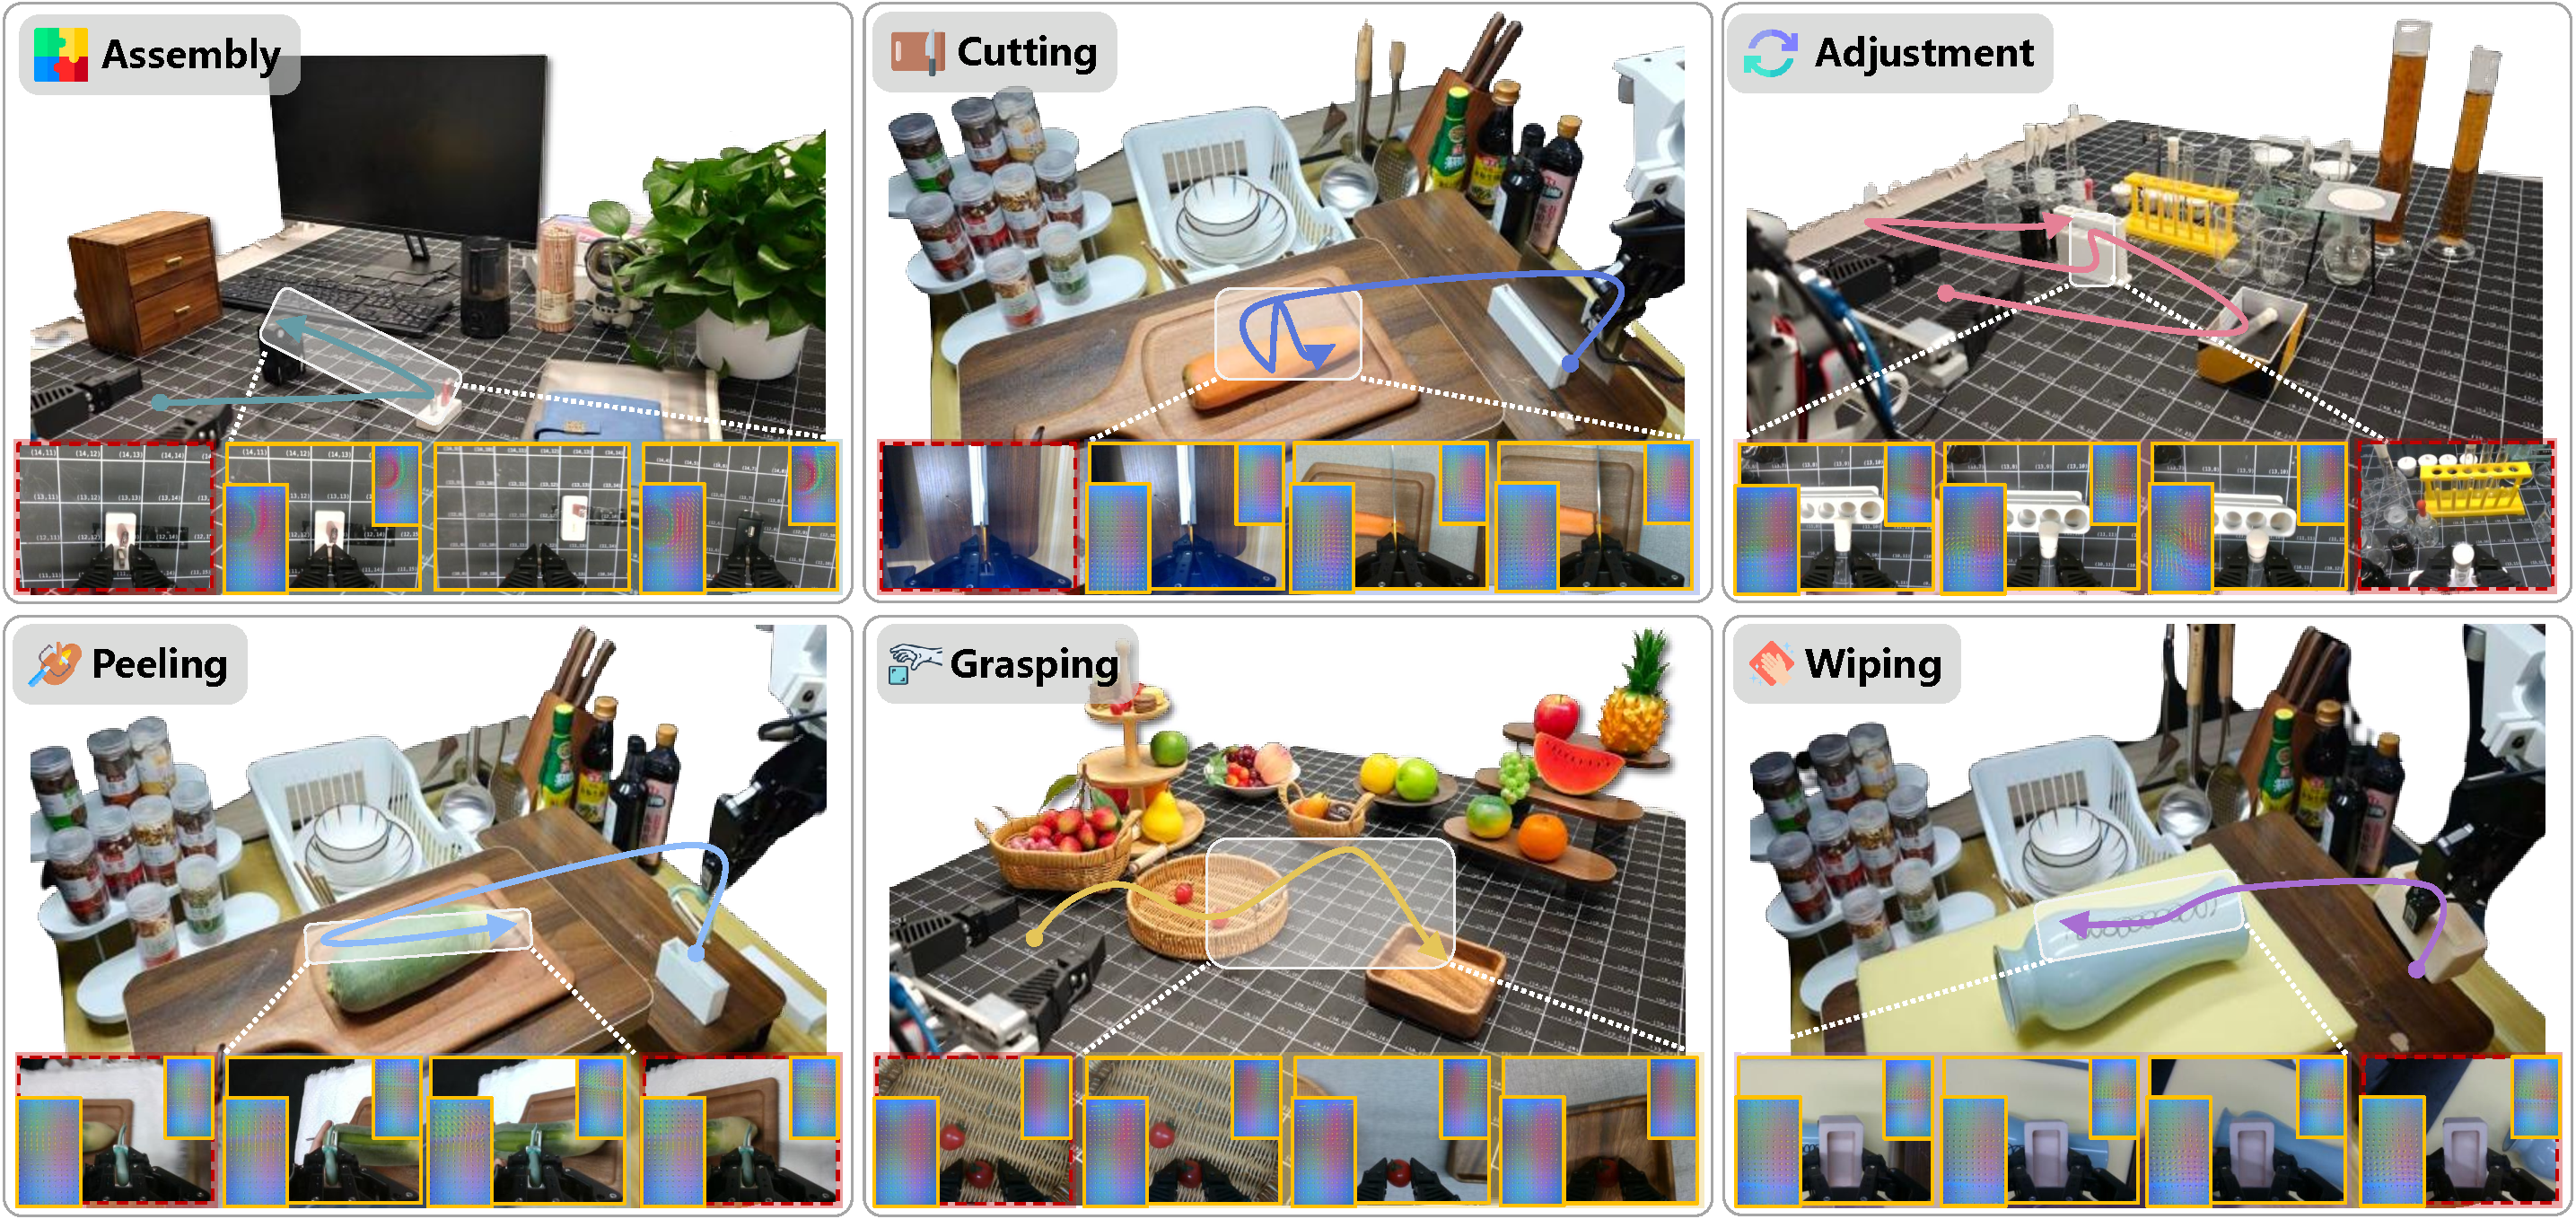
\includegraphics[width=0.95\linewidth]{fig/OmniVTA-6pattern.pdf}
\caption{\textbf{Example visualization of the $6$ visuo-tactile manipulation patterns in OmniViTac.} The dataset captures diverse, contact-rich behaviors across various scenarios, including Assembly, Cutting, Adjustment, Peeling, Grasping, and Wiping. Each panel illustrates the global third-person workspace view overlaid with the end-effector's trajectory, alongside synchronized, high-frequency tactile maps (bottom) that continuously record the complex tool-object contact dynamics during task execution.}
\label{fig:show_case}
\end{figure*}

\subsection{Hardware Setup and Data Collection System}
\label{sec:hardware}

\subsubsection{System Overview}

To efficiently collect large-scale visuo-tactile manipulation data, we develop a unified multimodal data acquisition system that can be operated by a single human operator. The system records synchronized multimodal observations during manipulation, including RGB-D visual observations, tactile signals from fingertip sensors, manipulation trajectories, and continuous gripper aperture states.

All sensory streams are recorded asynchronously at their native frequencies. A post-processing synchronization pipeline then aligns different modalities using timestamps to ensure consistent temporal correspondence across all observations.

\subsubsection{Dual-Embodiment Data Collection}

To balance \emph{robot-aligned demonstrations} and \emph{data collection scalability}, our dataset is collected using two complementary hardware embodiments: a 7-DoF robotic manipulator (xArm-7) and a TacUMI handheld data collection device. The robotic platform captures demonstrations that closely match the kinematic and dynamic distributions of robot execution, while TacUMI enables flexible and efficient human manipulation for large-scale data collection.

\noindent \textbf{Robot Demonstrations (7DoF Robot Arm).}
We employ a {UFACTORY xArm-7} manipulator to collect robot-aligned demonstrations. Two control modes are used:

\begin{itemize}
\item \textbf{Kinesthetic Teaching.} The operator directly guides the robot under gravity compensation mode, allowing precise control of contact interactions. This mode is particularly suitable for tasks requiring fine force perception, such as wiping surfaces or inserting connectors.

\item \textbf{GELLO Teleoperation.} For tasks involving larger spatial motions and less reliance on direct force perception, we adopt the {GELLO teleoperation system}~\cite{wu2024gello}. This master–follower interface enables efficient collection of pick-and-place style demonstrations while preserving realistic robot motion trajectories.
\end{itemize}

\begin{table*}[thb!]
    \centering
    \captionsetup{width=\textwidth}
    \caption{\textbf{Comparison of OmniViTac with existing vision-tactile-action datasets.} \textit{Note:} * indicates that the statistics count only the visuo-tactile trajectories in the corresponding dataset. ``--" denotes not applicable.
    } 
    \label{tab:dataset_comparison} 
    \vspace{-2mm}
    \addtolength{\tabcolsep}{-2pt}
    \resizebox{\textwidth}{!}{
        \begin{tabular}{@{}lccccccccc@{}}
            \toprule
            \multirow{2}{*}{\textbf{Dataset}} & \multirow{2}{*}{\textbf{\#Task}} & \multirow{2}{*}{\textbf{\#Traj.}} & \multirow{2}{*}{\textbf{\#Object}} & \multirow{2}{*}{\textbf{Vision}} & \multicolumn{3}{c}{\textbf{Tactile}} & \multirow{2}{*}{\textbf{Action}} & \multirow{2}{*}{\textbf{Collection}} \\ \cmidrule(lr){6-8}
             &  &  &  &  & \textbf{Sensors} & \textbf{Force Dim.} & \textbf{Frequency} &  &  \\ \midrule
            ObjectFolder2.0~\cite{gao2022objectfolder} & 3 & -- & 1,000 & Rendered & GelSight & 3 & -- & \xmark & Simulated \\
            AnyTouch~\cite{feng2025anytouch} & 1 & -- & 124 & -- & GelSight Mini/DIGIT/DuraGel/Tac3D & 3 & 30 & \xmark & Handheld \\
            VTV150k~\cite{xie2025universal} & -- & -- & 100 & -- & GelSight Mini/DIGIT/Tac3D & -- & -- & \xmark & Handheld \\
            Octopi-1.5~\cite{yu2025demonstrating} & 3 & -- & -- & GoPro & GelSight Mini/TAC-02 & -- & 50$\sim$1000 & \cmark & TMI \\
            See, Hear, and Feel~\cite{li2022see} & 2 & 60 & 4 & RealSense & GelSight & -- & 30 & \cmark & Teleop \\
            RH20T*~\cite{fang2023rh20t} & 55 & 917 & -- & RealSense & uSkin & -- & 200 & \cmark & Teleop \\
            FreeTacMan~\cite{wu2025freetacman} & 50 & 10,000 & 50 & Fisheye & FreeTacMan & -- & 30 & \cmark & Fingertips \\
            VLA-Touch~\cite{bi2025vla} & 3 & -- & -- & RealSense & GelSight Mini & -- & 10 & \cmark & Kinesthetic Teaching \\
            OmniVTLA~\cite{cheng2025omnivtla} & 2 & 240 & 56 & RealSense & GelSight/Paxini Gen 2 & -- & 30 & \xmark & Handheld \\
            exUMI~\cite{xu2025exumi} & 9 & 1,665 & 8 & GoPro & 9DTact & 6 & -- & \cmark & UMI-style \\
            MLA~\cite{liu2025mla} & 6 & 1,200 & 14 & RealSense & Tashan TS-E-A & 6 & -- & \xmark & Gello-teleop \\
            Hoi!~\cite{engelbracht2025hoi} & 6 & $\sim$3,000 & 381 & Zed Mini/Aria & DIGIT & 6 & 30$\sim$60 & \cmark & Gello-teleop \\
            AgiBot World*~\cite{bu2025agibot} & 7 & 5,337 & -- & -- & Xense & 3 & -- & \cmark & Teleop \\ \midrule
            \textbf{OmniViTac (Ours)} & 86 & 21,879 & 126 & RealSense/Fisheye & Xense/Gelsight Mini/DM-Tac/Tac3D & 3 & 30$\sim$60 & \cmark & UMI-style/Kinesthetic Teaching \\ \bottomrule
        \end{tabular}}
    \vspace{-5mm}
    \addtolength{\tabcolsep}{2pt}
\end{table*}

\noindent \textbf{Human Demonstrations (TacUMI).} 
To improve data collection efficiency and flexibility, we develop {TacUMI}, a handheld visuo-tactile data collection device inspired by FastUMI~\cite{zhaxizhuoma2025fastumi}. TacUMI enables natural manipulation motions while recording multimodal sensory observations that are consistent with the robotic platform. Following FastUMI, we use a {RealSense T265} tracking camera, which outputs 6-DoF poses at 200~Hz to estimate trajectories. After each trajectory is collected, an automatic verification step checks for tracking drift, and trajectories with position errors larger than 8~mm are discarded.



\noindent \textbf{Isomorphic End-Effector.}
To minimize embodiment-induced domain gaps, both the robotic arm and TacUMI employ identical parallel-jaw grippers. This shared end-effector design ensures consistent grasp geometry and contact mechanics across both data collection embodiments. Each gripper records \emph{continuous motor states}, which are normalized to a $[0,1]$ range to represent the gripper width. The fingertip structure is modular and supports interchangeable tactile sensor modules.

\subsubsection{Sensor Suite}
To capture the diverse perceptual cues required in contact-rich manipulation, we combine RGB-D sensing with multiple tactile sensors that provide complementary observations of object geometry, surface interaction, and contact dynamics.

\noindent \textbf{Visual Observation.}
We record both \emph{wrist-view} and \emph{third-person-view} RGB-D observations. Wrist-view images are captured using an Intel RealSense D435 camera, while third-person observations are captured using either a D435 or an L515 camera. All cameras record RGB-D streams at 30~Hz. The D435 provides images at $640\times480$ resolution, while the L515 provides $1280\times720$ resolution. TacUMI additionally integrates a wide-angle RGB camera to capture broader environmental context.

\noindent \textbf{Tactile Sensing.}
Tactile sensors are mounted on the gripper fingertips to capture detailed contact information during manipulation. Our platform supports four types of tactile sensors with different sensing principles and resolutions:

\begin{itemize}

\item \textbf{Xense (Quark N1):}
records RGB tactile images with a resolution of $700\times400$ at 30~Hz and 3D displacement fields with a spatial resolution of $35\times20$ at 60~Hz.

\item \textbf{Daimon (Tac-WL):}
records grayscale tactile images at $640\times480$ resolution at 30~Hz and 3D displacement measurements with resolution $320\times240$ at 60~Hz.

\item \textbf{Tac3D-A1:}
provides dense 3D displacement sensing with spatial resolution $20\times20$ at 30~Hz.

\item \textbf{GelSight Mini:}
records RGB tactile images with resolution $320\times240$ and 3D displacement fields with spatial resolution $9\times7$, both captured at 25~Hz.

\end{itemize}

These sensors provide multiple tactile signal modalities for the same manipulation tasks. The Xense sensor is used for the majority of data collection due to its robustness in large-scale manipulation datasets. 
Consequently, demonstrations collected with Xense are primarily used for analysis and real-robot evaluation, while the additional tactile sensors are included to support research on tactile representation learning and cross-sensor generalization.

\noindent \textbf{Proprioceptive Signals.}
The system also records proprioceptive states, including robot joint states (only for xArm demonstrations), end-effector poses, and continuous gripper aperture values. During data collection, the average tactile displacement is visualized in real time to provide operators with an intuitive estimate of contact forces.

\subsubsection{Data Collection and Processing Pipeline}
We describe how visuo-tactile-action trajectories are recorded and how the raw data are collected, validated, and processed.

\noindent \textbf{Data Acquisition.}
To enable single-operator data collection, we design a foot-pedal control interface for managing the entire recording process. The interface provides three functions: starting the system, recording trajectories, and stopping it. During recording, all sensors continuously publish timestamped observations, which are subscribed and stored by the host computer. To prevent sensor drift from extended operation, the system automatically restarts after every 25 trajectories.

\noindent \textbf{Data Validation.}
We perform both online and offline quality checks. During collection, every 50 trajectories the system randomly selects three trajectories and visualizes synchronized sensor streams, including camera observations, tactile signals, trajectory curves, and gripper width signals. After data collection, all trajectories can be inspected offline using visualization tools, and abnormal samples are removed.

\noindent \textbf{Data Processing.}
Before policy training, we preprocess all trajectories to improve data quality and temporal consistency. This pipeline removes redundant static frames at the beginning and end of each trajectory, aligns RGB-D, tactile, and action streams through timestamp synchronization (with temporal error below 10~ms), and segments trajectories into training-ready clips according to downstream policy learning requirements.


\begin{figure*}[ht]
\centering
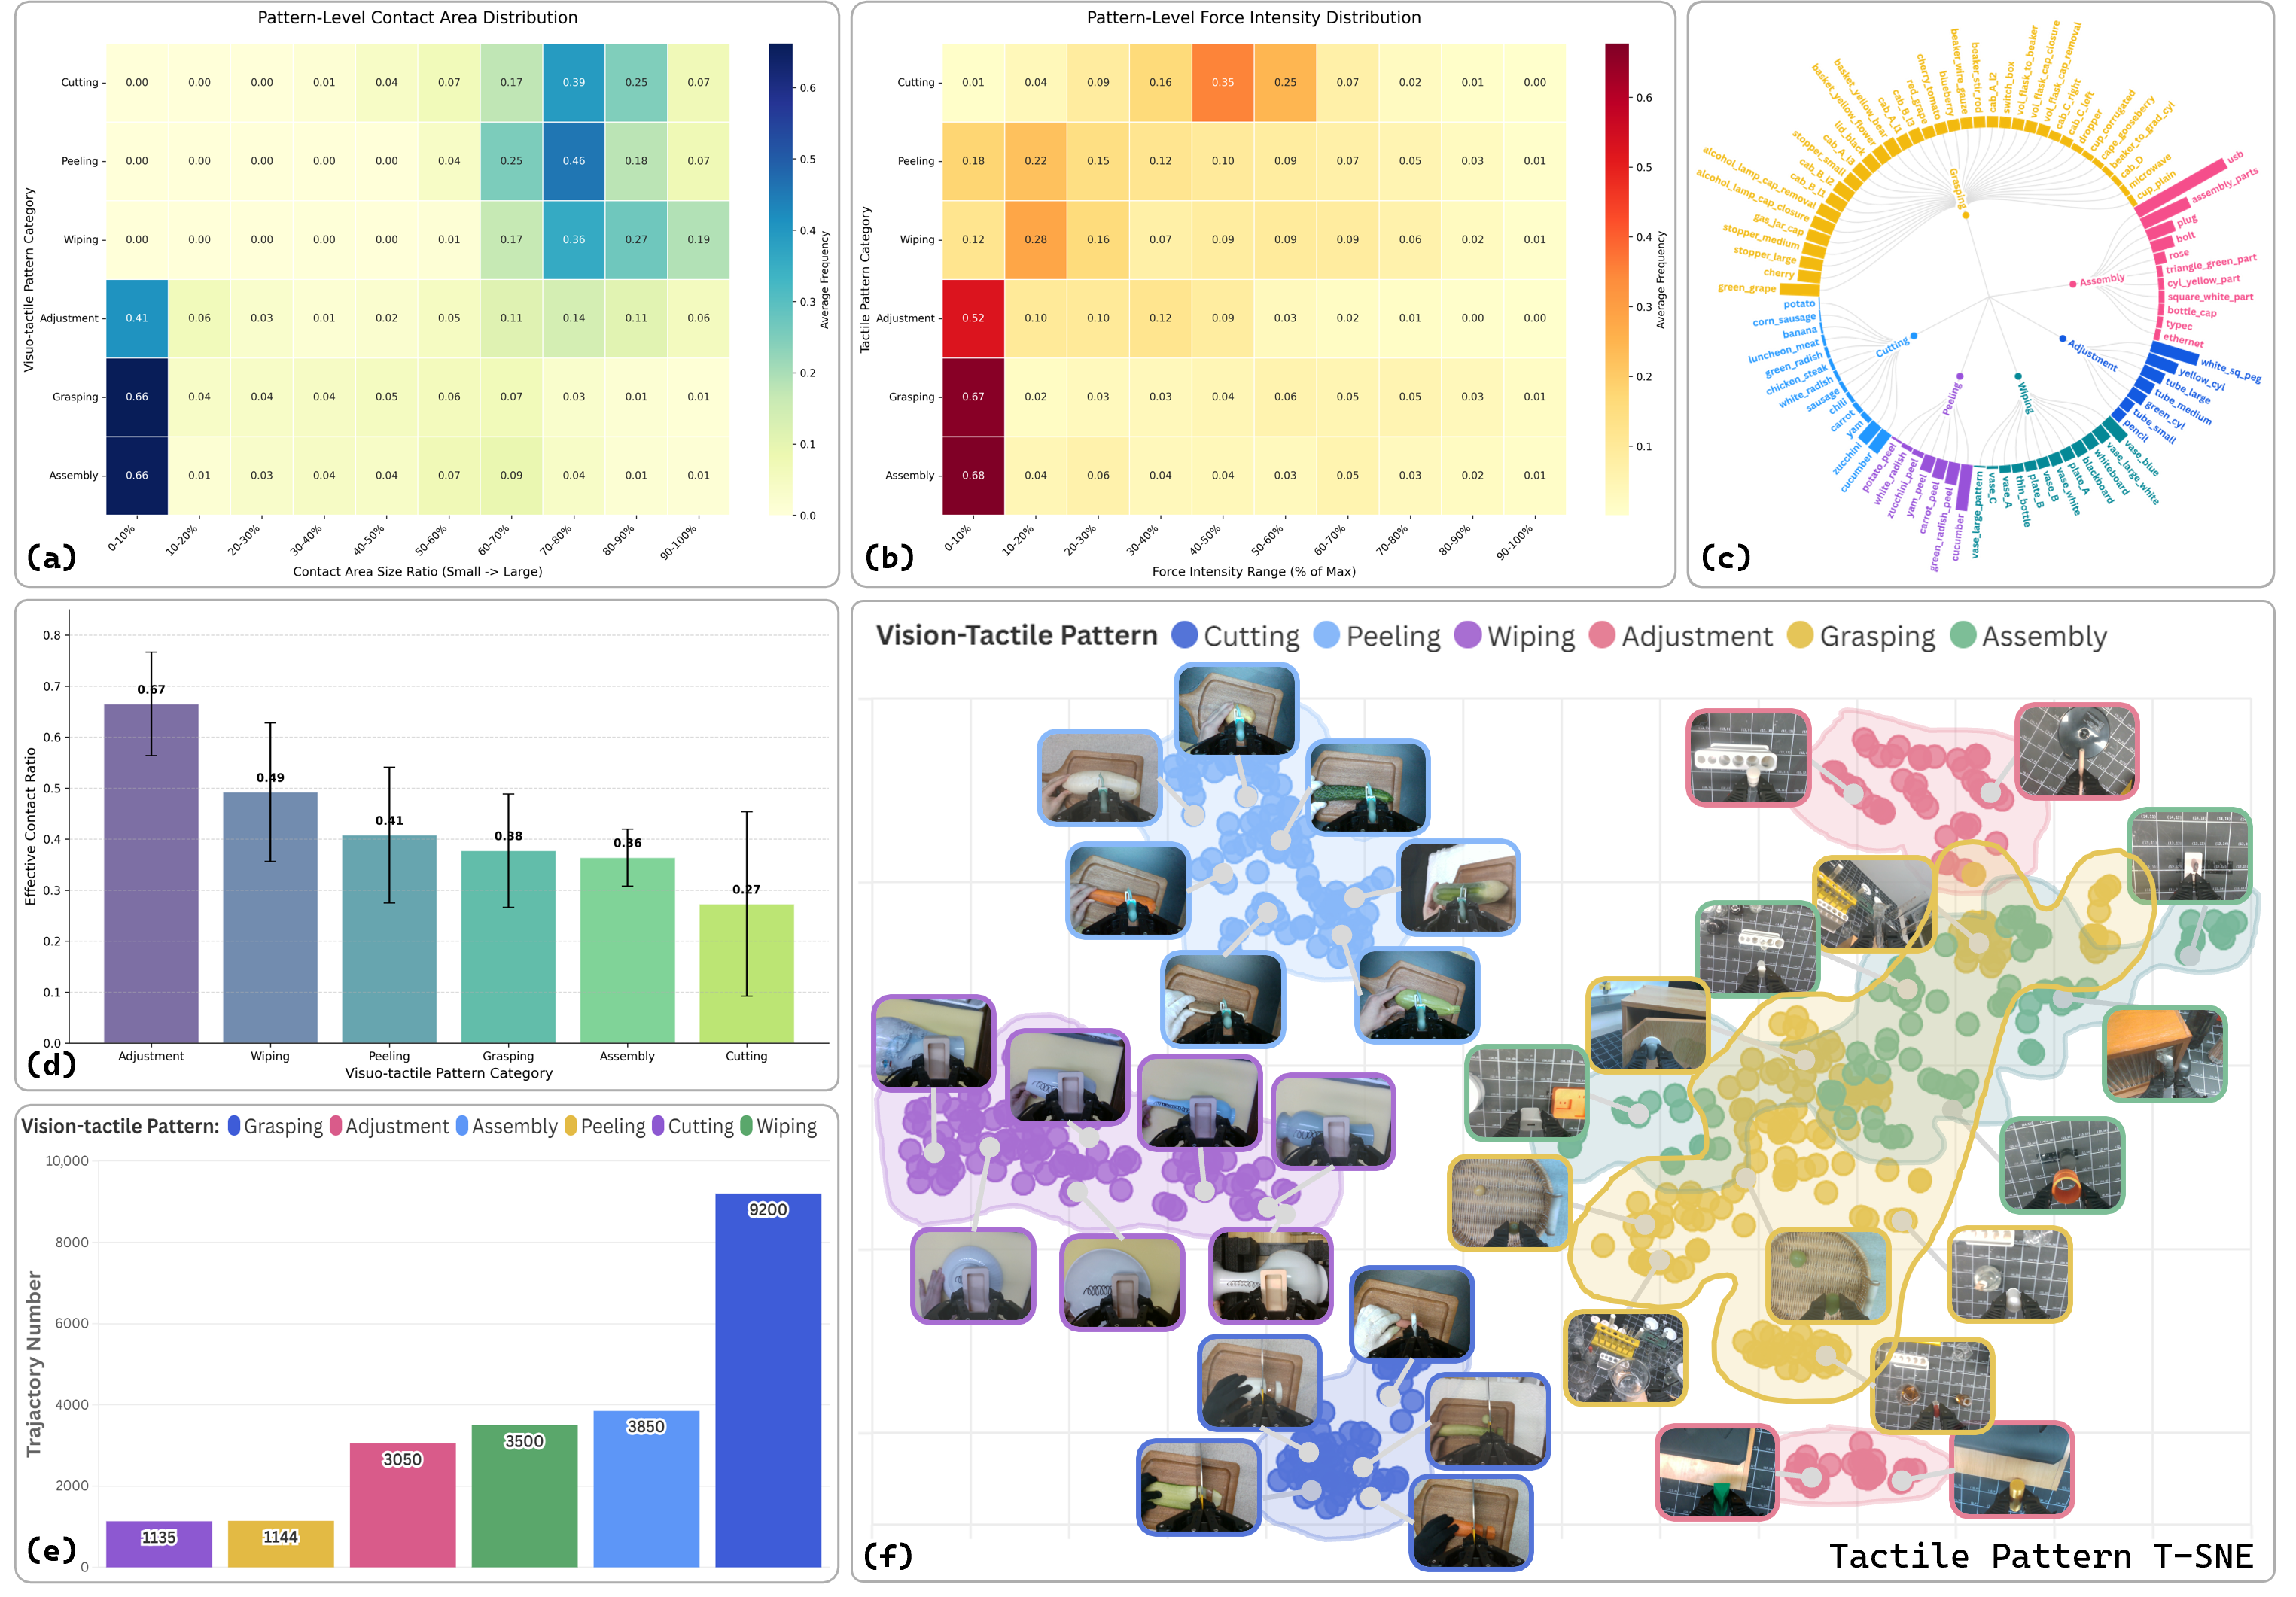
\includegraphics[width=0.95\linewidth]{fig/data_stat_family.png}
\caption{\textbf{{Comprehensive statistical analysis of the OmniViTac.}} 
\textbf{(a)} Pattern-level contact area distribution, highlighting the distinct dichotomy between precision-dominant tasks (concentrated in the $0$-$10\%$ range) and surface-dominant tasks (peaking at $70$-$90\%$). 
\textbf{(b)} Force intensity distribution, showcasing the wide spectrum of force magnitudes required across different manipulation modes. 
\textbf{(c)} Hierarchical distribution illustrating the rich diversity of $86$ instantiated tasks. 
\textbf{(d)} Effective contact ratio with variance across patterns, demonstrating the temporal dependency on tactile feedback (e.g., \textit{Adjustment} exhibits the highest continuous engagement). 
\textbf{(e)} Total trajectory counts per category, demonstrating the massive scale and balanced composition of the benchmark. 
\textbf{(f)} t-SNE projection of the high-dimensional tactile signals, revealing physically intuitive and semantically separable latent clusters that strictly align with the underlying contact mechanics of each interaction pattern.}
\label{fig:statistic}
\end{figure*}



\subsection{Task Taxonomy and Tactile Pattern Analysis}
\label{sec:task}
\subsubsection{Environmental Diversity}

To facilitate robust generalization of visuo-tactile policies to real-world environments, OmniViTac is deliberately designed with high environmental diversity. As illustrated in the inner ring of Fig.~\ref{fig:dataset_teaser} and the examples in Fig.~\ref{fig:show_case}, the dataset encompasses over 70 distinct manipulation tasks, systematically distributed across five semantic scenarios: \textit{Kitchen, Fruit Shop, Industrial Workspace, Chemistry Laboratory,} and \textit{Office}. Diverse scene selection ensures broad coverage of visual distractors, varying illumination conditions, and a wide range of object properties, including rigid, deformable, transparent, and articulated types, thereby posing fundamental challenges to the robustness of policies.


\subsubsection{Task Taxonomy}
To move beyond task classification based purely on visual kinematics, we introduce a physics-grounded taxonomy that categorizes the collected behaviors into six representative visuo-tactile patterns. This taxonomy is defined by the dominant tactile features and contact mechanics underlying successful execution:
\begin{itemize}
    \item \textbf{Assembly:} Involves precise coordination of contact geometry and multi-directional forces to perceive tight tolerances and detect successful mating of intricate parts.
    \item \textbf{Cutting:} Predominantly relies on the progressive magnitude of normal forces to penetrate objects, using sudden force drops to judge the completion of the severing action.
    \item \textbf{Adjustment:} Characterized by torsional and shear forces, which are crucial for sensing slip and reorienting in-hand objects until the desired stable pose is achieved.
    \item \textbf{Peeling:} Involves a dynamic and continuous coupling of both shear and normal forces to maintain constant tool-surface contact while stripping object exteriors.
    \item \textbf{Wiping:} Another canonical contact-rich task demanding the simultaneous regulation of normal pressure (to maintain surface adherence) and planar shear force (to overcome friction during sweeping motions).
    \item \textbf{Grasping:} A highly versatile category encompassing a broad spectrum of force profiles. It utilizes precise normal force control to safely handle fragile items, leverages contact feedback to verify secure holds on visually challenging (e.g., transparent) objects, and exploits combined normal-shear dynamics to optimize the manipulation of complex articulated mechanisms.
\end{itemize}



\subsubsection{Tactile Pattern Analysis}

To quantitatively validate the proposed task taxonomy and analyze the underlying data distribution, we embed the high-dimensional tactile signals from all six pattern categories into a two-dimensional latent space using t-SNE, as shown in Fig.~\ref{fig:statistic}(f). The embedding reveals a highly structured and physically interpretable distribution. Notably, tasks dominated by continuous, high-frequency shear and dynamic normal forces, such as \textit{Wiping} and \textit{Peeling}, form overlapping or closely adjacent clusters, reflecting their shared underlying contact mechanics. In contrast, tasks governed primarily by static normal pressure and localized geometric contacts, such as \textit{Assembly}, yield distinct and well-separated manifolds. The \textit{Grasping} category occupies a broad and expansive region in the feature space, consistent with its inherent intra-class diversity spanning delicate handling of fragile objects to manipulation of complex articulated mechanisms. This clear semantic separability within the tactile latent space underscores that OmniViTac captures rich, pattern-specific contact dynamics rather than redundant or noisy signals.



\subsection{Dataset Statistics and Scale}
\label{sec:statistics}

\subsubsection{Overview Statistics}
% zyp modify
To rigorously benchmark the scale, diversity, and fidelity of OmniViTac, we provide a comprehensive statistical analysis of all collected trajectories, with an emphasis on task distributions and their associated spatio-temporal tactile properties.
As illustrated in Fig.~\ref{fig:statistic}(e), the dataset captures a broad range of visuo-tactile patterns commonly encountered in daily manipulation tasks. The ``grasping" category constitutes the largest subset, comprising 9,200 trajectories. Other manipulation categories also account for a significant portion of the dataset, each comprising approximately 3,000 or 1,000 trajectories, with all categories remaining within the same order of magnitude. This balanced composition ensures sufficient data density for both general-purpose pre-training and task-specific fine-tuning.




\subsubsection{Tactile Active Ratio}

A key metric for evaluating contact-rich datasets is the Effective Contact Ratio, defined as the proportion of a trajectory during which the tactile sensors register meaningful tactile interaction. As shown in Fig.~\ref{fig:statistic}(d), \textit{Adjustment} exhibits the highest active ratio (0.67) with relatively low variance, primarily because in-hand reorientation demands continuous contact with the tool or object to monitor slip and state changes. Similarly, tasks such as \textit{Wiping} (0.49) and \textit{Peeling} (0.41) require prolonged frictional interaction. In contrast, \textit{Cutting} yields the lowest active ratio (0.27) and exhibits high variance, as these patterns typically involve an extended phase of visual alignment and pre-contact approach before the brief, high-force severing event.

\subsubsection{Pattern-level Contact Area and Force Intensity}

The heatmaps in Fig.~\ref{fig:statistic}(a) and (b) reveal a clear and physically intuitive distinction in how tactile sensors are spatially and dynamically engaged across different manipulation patterns.

\begin{itemize}
\item \textbf{Precision-oriented tasks} (e.g., \textit{Assembly, Grasping, Adjustment}): These manipulations are predominantly associated with the lowest deciles in both contact area (with $66\%$ of occurrences in the $0-10\%$ range) and force intensity. This distribution reflects the underlying nature of these tasks, which rely on delicate, localized fingertip contacts and sensitive low-magnitude force feedback to adjust object poses or prevent damage precisely.
\item \textbf{Power-oriented or surface-oriented tasks} (e.g., \textit{Cutting, Peeling, Wiping}): In contrast, these tasks exhibit extensive sensory activation. Their contact area distributions peak prominently in the $70\%-90\%$ range, indicating full-patch engagement of the sensor surface to maintain frictional contact. Moreover, \textit{Cutting} shows a marked shift toward higher force intensities (peaking in the $40\%-50\%$ range of sensor capacity), which is necessary for penetrating materials and overcoming physical resistance.
\end{itemize}

Together, these multi-dimensional statistics demonstrate that OmniViTac is not merely a collection of random contacts, but a highly structured and physically grounded benchmark, well-suited to support advanced research in visuo-tactile perception and contact-rich policy learning.
\begin{figure*}[ht]
\centering
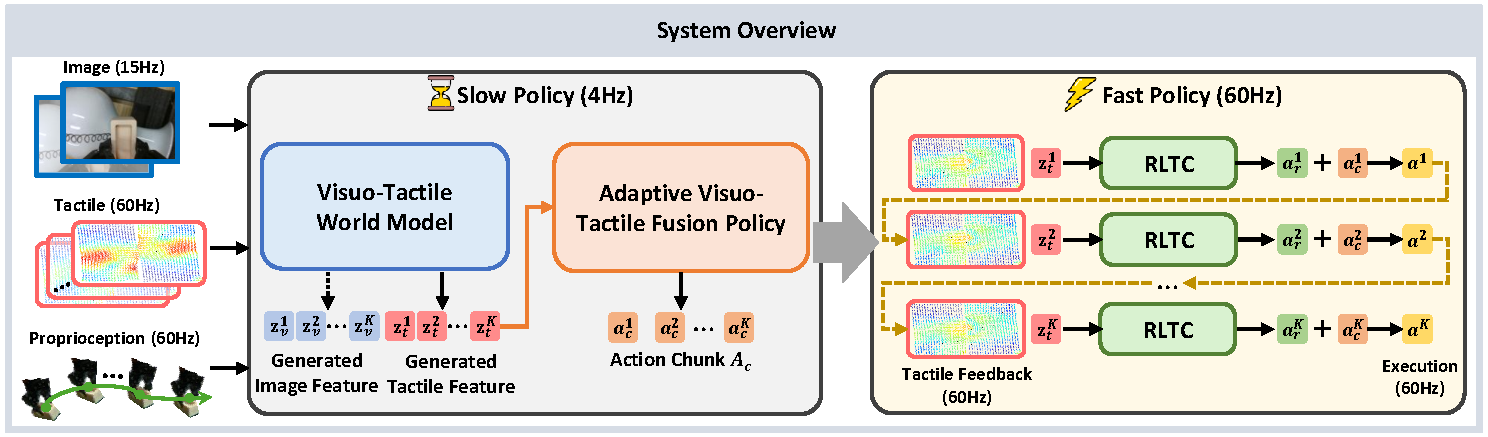
\includegraphics[width=0.95\linewidth]{fig/system.pdf}
\caption{\textbf{{System Overview}}. OmniVTA is a hierarchical slow–fast policy for contact-rich manipulation. The slow policy contains a visuo-tactile world model and an adaptive fusion policy to generate long-horizon action chunks from multi-modal inputs. 
The fast policy outputs high-frequency refinements at $60$~Hz using tactile feedback. 
Final actions are a weighted summation of slow-planned and fast-refined outputs, enabling both long-horizon planning and reactive control for robust manipulation.}
\label{fig:system}
\end{figure*}

\section{Methodology}



\subsection{System Overview}
To achieve stable and robust contact-rich manipulation, we introduce {OmniVTA}, a hierarchical slow-fast manipulation policy built upon a visuo-tactile world model, as illustrated in Fig.~\ref{fig:system}. OmniVTA explicitly decomposes manipulation into \emph{slow planning} and \emph{fast reflexive control}. 
The \emph{Slow Policy} integrates the Visuo-Tactile World Model (VTWM) and the Adaptive Visuo-Tactile Fusion Policy (AFP) to perform long-horizon action chunk planning from low-frequency visual observations, high-frequency tactile signals, and proprioceptive states. To improve efficiency, the world model predicts future tactile signals without generating visual observations during inference, enabling higher-frequency rollout while preserving contact-relevant dynamics.
The \emph{Fast Policy} is implemented as a Reflexive Latent Tactile Controller (RLTC), inspired by the reflexive control paradigm~\cite{xu2025aprebot, xu2025rebot}, which outputs fine-grained corrective actions at 60~Hz based on both predicted and observed tactile signals. This controller refines the action sequences generated by the slow policy by combining the planned actions with the controller outputs through a weighted summation, where the controller contribution is scaled by a predefined coefficient before execution on the robot.
This slow-fast decomposition enables both long-horizon planning and high-frequency reflexive control, which are critical for contact-rich manipulation.

In the following, we detail the components of OmniVTA. Sec.~\ref{sec:tacvae} introduces the TactileVAE for tactile feature extraction. Sec.~\ref{sec:vtwm} presents the Visuo-Tactile World Model, which captures contact dynamics via joint visual-tactile prediction. Sec.~\ref{sec:fusion_policy} describes the adaptive fusion policy with a gated mechanism~\cite{cao2023multi} for integrating visual and tactile features. Sec.~\ref{sec:controller} details the Reflexive Latent Tactile Controller.



\subsection{TactileVAE}
\label{sec:tacvae}
TactileVAE aims to rapidly extract low-dimensional, continuous, and task-agnostic tactile representations for downstream prediction and policy learning. For optical tactile sensors, instead of using high-resolution tactile images, we adopt \textit{3D marker displacement} as tactile input. This representation captures contact-induced surface deformation while maintaining significantly lower resolution, enabling efficient feature extraction and higher-frequency inference. The structure of the TactileVAE is shown in Fig.~\ref{fig:vae}, which contains a spatial-temporal encoder and an implicit deformation decoder.

\subsubsection{Encoder}
We construct a spatio-temporal encoder to extract compact tactile token representations. Since the markers on the tactile surface are uniformly distributed, a single-frame tactile observation can be represented as a tensor of size $H \times W \times 3$ where $H$ and $W$ denote the number of markers along the $y$- and $x$-axes, respectively, and the channel dimension corresponds to the marker displacement along the $x$, $y$, and $z$ directions.

As tactile sensing typically operates at a higher frequency than vision, we perform joint temporal and spatial compression to reduce the number of tactile tokens and align them with visual tokens in time. To this end, we adopt a \textit{3D convolution-based variational autoencoder (VAE)} and pretrain it on a large corpus of real tactile data to learn low-dimensional, task-agnostic latent features.

As illustrated in Fig.~\ref{fig:vae}, the encoder consists of a projection-in layer (causal 3D convolution), $M$ downsampling modules, and a projection-out layer (causal 3D convolution). The input is encoded into a latent feature map of size $\frac{H}{s} \times \frac{W}{s} \times C$, where $s = 2^M$ is the spatial downsampling factor and $C$ is the latent dimension. We adopt \textit{causal 3D convolutions} along the temporal axis so that the latent representation at time $t$ depends only on current and past observations, ensuring consistency between training and real-time deployment.

\subsubsection{Decoder}

Instead of reconstructing pixels as in conventional VAEs, we employ an \textit{implicit neural representation (INR)}~\cite{sitzmann2020implicit} decoder to model a continuous tactile deformation field conditioned on spatial coordinates. Implicit representations are well-suited for modeling continuous signals and have been widely used in computer vision tasks such as geometric reconstruction~\cite{zhong20233d, park2019deepsdf} and dense prediction~\cite{chen2023dpf, yu2026infinidepth}. Since marker displacement arises from the continuous deformation of the elastomer surface under contact, we model the deformation field as a continuous function:

\begin{equation}
    \mathbf{d}(\mathbf{x}) = \mathcal{D}_{\theta} \left( \gamma(\mathbf{x}), \Phi(\mathbf{z}_{t}, \mathbf{x}) \right),
\end{equation}
where $\mathbf{x} \in \mathbb{R}^2$ denotes the spatial coordinate, $\mathbf{z}_{t}$ is the latent feature map, $\gamma(\cdot)$ represents positional encoding, $\Phi(\mathbf{z}_{t},\mathbf{x})$ retrieves local features from $\mathbf{z}_{t}$ via spatial interpolation, and $\mathcal{D}_{\theta}$ is an MLP decoder that predicts the 3D deformation $\mathbf{d}(\mathbf{x}) \in \mathbb{R}^3$. 
During training, we uniformly sample query points in the latent feature map and extract their local features, which, together with the corresponding positional encodings, are fed into the decoder to predict the corresponding \textit{3D deformation vector}. This yields a continuous reconstruction of the tactile surface deformation field.
% During training, we uniformly sample query points within the latent feature map and extract the corresponding local features. Together with the positional encoding of the query coordinates, these features are fed into the decoder to predict the corresponding \textit{3D deformation vector}, thereby reconstructing the continuous deformation field of the tactile surface.

\subsubsection{Training Loss}
For supervision, the ground-truth deformation $\hat{\mathbf{d}}(\mathbf{x})$ at each query point $\mathbf{x}$ is obtained by interpolating the original 3D deformation. 
The TactileVAE is trained with a reconstruction loss and a KL regularization term~\cite{kingma2013auto}:

\begin{equation}
\mathcal{L}_{\text{TacVAE}} 
= \|\mathbf{d}(\mathbf{x}) - \hat{\mathbf{d}}(\mathbf{x})\|_2^2
+ \lambda_{\mathrm{KL}} \, \mathcal{L}_{\mathrm{KL}}.
\end{equation}

\begin{figure}[t]
\centering
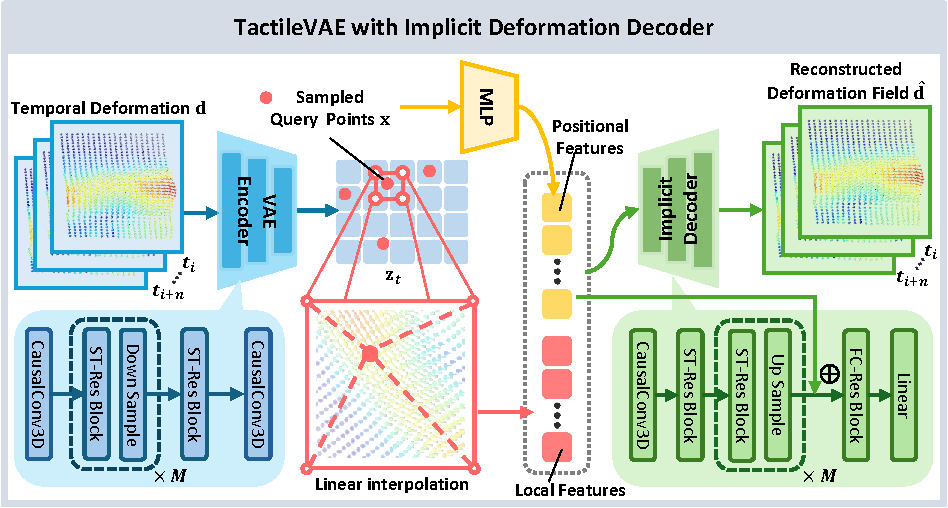
\includegraphics[width=\linewidth]{fig/vae.pdf}
\caption{\textbf{Overview of TactileVAE.} The model encodes 3D marker displacements into spatio-temporal features, and reconstructs the deformation via an implicit decoder that represents the deformation as a continuous field.}
\label{fig:vae}
\end{figure}


\begin{figure*}[ht]
\centering
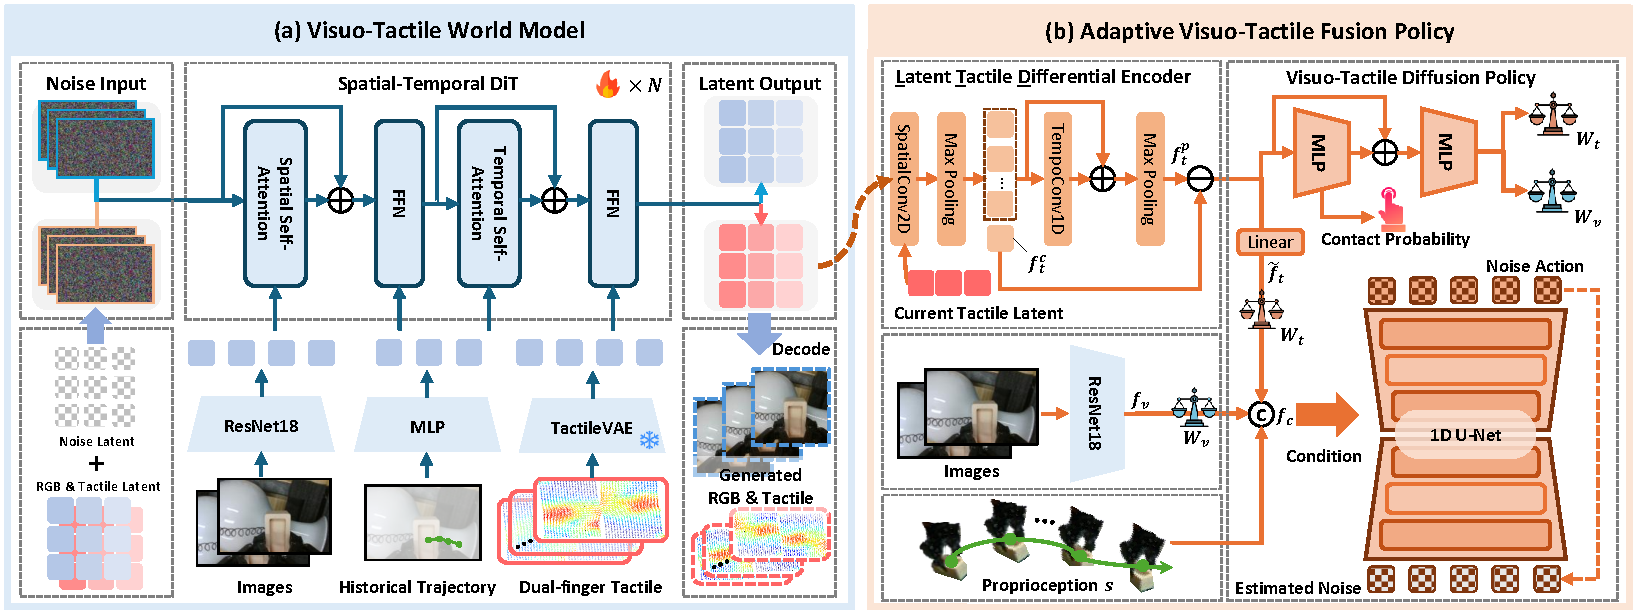
\includegraphics[width=0.95\linewidth]{fig/slow-policy.pdf}
\caption{\textbf{Overview of the Slow Policy.} \textbf{(a):} The proposed Visuo-Tactile World Model takes noisy tactile and visual latent sequences as input and jointly generates both modalities via a two-stream spatio-temporal diffusion transformer. \textbf{(b):} The Adaptive Visuo-Tactile Fusion Policy employs a Latent Tactile Differential Encoder to effectively encode the observed and predicted tactile and a gating mechanism to adaptively balance tactile and visual information for robust action planning.}
\label{fig:slow_policy}
\vspace{-5mm}
\end{figure*}

\vspace{-5mm}
\subsection{Visuo-Tactile World Model}
\label{sec:vtwm}
In this section, we present the Visuo-Tactile World Model, which adopts a two-stream conditional generative framework and explicitly models the temporal evolution of visual observations and tactile signals, thereby learning a dynamic prior for multimodal interactions. Overall, it consists of three key modules. The two-stream world model separately characterizes the dynamic generation process of the visual and tactile modalities while performing coordinated prediction under a shared condition. The multimodal observation conditioner jointly encodes vision, tactile, and actions, providing consistent conditioning for the generation process. The dynamic-aware weighted loss further emphasizes regions with high-frequency tactile variations and salient contact responses, improving the modeling of fine-grained tactile dynamics.

\subsubsection{Two-stream World Model}
To model the evolution of visual observations and tactile states during policy execution, we build a two-stream visuo-tactile world model, as shown in Fig.~\ref{fig:slow_policy} (a). Both branches employ a spatial-temporal diffusion transformer~\cite{peebles2023scalable}, which stacks transformer blocks along temporal and spatial axes. Specifically, the model takes the past $c$ frames as conditioning and iteratively denoises to generate multiple future frames, yielding a probabilistic model of future dynamics. The diffusion objective is defined as

\vspace{-2mm}
\begin{equation}
\mathcal{L}_{\text{diffusion}}=\mathbb{E}_{\mathbf{z}_o, \boldsymbol{\epsilon}, t}\left[\sum_{i=1}^K \left(1-m_i\right) \odot \left\|\epsilon_i-\boldsymbol{\epsilon}_\theta\left(\mathbf{z}_o, t\right)_i\right\|_2^2\right],
\end{equation}
where $\mathbf{z}_o = \left\{ \mathbf{z}_o^{1}, \dots, \mathbf{z}_o^{K} \right\}$ denotes a sequence of observation latents (including tactile latent $\mathbf{z}_t$ and visual latent $\mathbf{z}_v$), and $\boldsymbol{\epsilon}_\theta(\mathbf{z}_o, t)$ predicts the noise for the entire sequence. Each $\mathbf{z}_o^{i}$ corresponds to the encoded observation at timestep $i$. The mask $m$ provides temporal conditioning, encouraging the model to leverage historical observations for predicting future states.
At the modality encoding layer, the visual branch uses an SD-VAE~\cite{rombach2022high} to extract image latents, while the tactile branch employs the TactileVAE pretrained in the previous stage to compress tactile signals. After obtaining the latent representations of vision and touch, the two modalities are fed into their corresponding spatial-temporal diffusion models, enabling parallel modeling and joint generation. 

\subsubsection{Multi-modal Observation Conditioner}
To model joint visual-tactile dynamics effectively, we design a multi-modal conditional encoder for visual-tactile-action interactions. This module first performs feature extraction and temporal aggregation separately for visual observations, tactile embeddings, and action sequences, where each action is represented as the 2D image-plane projection of the 3D end-effector position. We observe that this representation improves robustness to variations in manipulation locations. The modalities are then fused in a shared linear projection space to produce a fixed-dimensional conditioning vector. This vector is injected as a shared prior into both the tactile and visual world models, aligning the two branches and improving cross-modal consistency during dynamic prediction.

\subsubsection{Dynamic-aware Weighted Loss}
To supervise high-frequency dynamic changes in tactile signals more effectively, we introduce a Dynamic-Aware Weighted Loss. Specifically, the loss constructs a dynamic weight map based on local temporal differences of the tactile sequence to capture time-varying activity at different spatial locations:
    \begin{equation}
    w_{\text{dyn}^{i}} =
    \operatorname{resize}\left(
    \operatorname{clip}_{[0,1]}
    \left(
    \left\|X_{i+1}-X_i\right\|_2
    \right)
    \right),
    \end{equation}
where $X_k$ denotes the tactile frame at the $k$-th timestep, and $\operatorname{resize}(\cdot)$ resizes the weight map from the raw tactile resolution to the latent resolution. The dynamic-aware loss is defined as the weighted simple diffusion loss:
        \begin{equation}
        \mathcal{L}_{\text{dyn}} =
        \mathbb{E}_{\mathbf{z}_o,\boldsymbol{\epsilon},t}
        \left[
        \sum_{i=2}^{K}
        w_{\text{dyn}}^{i}\odot(1-m_i)
        \odot
        \left\|
        \epsilon_{i}-\boldsymbol{\epsilon}_\theta(\mathbf{z}_o,t)_{i}
        \right\|_2^2
        \right].
        \end{equation}
In addition, an amplitude weight map is constructed from the response magnitude of the tactile signal to represent the distribution of local contact intensity:
\begin{equation}
w_{\text{amp}^{i}} =
\operatorname{resize}\left(
\operatorname{clip}_{[0,1]}
\left(
\left\|X_i\right\|_2
\right)
\right).
\end{equation}
The amplitude loss is defined as
\begin{equation}
\mathcal{L}_{\text{amp}}=\mathbb{E}_{\boldsymbol{z_o}, \boldsymbol{\epsilon}, t}\left[\sum_{i=2}^K w_{\text{amp}}^i \odot \left(1-m_i\right) \odot \left\|\epsilon_i-\epsilon_\theta\left(\mathbf{z}_{o}^{i}, t\right)\right\|_2^2\right],
\end{equation}
 
The two weight maps are then aligned to the spatial resolution of the tactile latent representation and jointly used to modulate the reconstruction loss during training. This weighting strategy explicitly highlights regions with rapid dynamics and strong contact responses during optimization, thereby improving the modeling of high-frequency tactile patterns, local contact changes, and fine-grained temporal structure.
Finally, the overall objective is a weighted sum of the diffusion loss and the dynamic-aware weighted loss:
    \begin{equation}
    \mathcal{L}_{VTWM}
    =
    \mathcal{L}_{\text{diffusion}}
    +
    \lambda_1 \mathcal{L}_{\text{dyn}}
    +
    \lambda_2 \mathcal{L}_{\text{amp}},
    \end{equation}
where $\lambda_1$ and $\lambda_2$ are the loss weights for the dynamic and amplitude terms, respectively.

\subsection{Adaptive Visuo-Tactile Fusion Policy}
\label{sec:fusion_policy}
We propose the Adaptive Visuo-Tactile Fusion Policy, which adaptively balances visual and tactile information based on the predicted contact state for stable action planning. The policy comprises three components: a Latent Tactile Differential (LTD) Encoder for tactile representation, an Adaptive Visuo-Tactile Fusion module for modality weighting, and a Visuo-Tactile Diffusion Policy for action generation.

\subsubsection{Latent Tactile Differential (LTD) Encoder}
Tactile signals exhibit strong spatial locality and remain largely inactive before contact, becoming informative only when physical interaction occurs. Previous approaches typically concatenate historical tactile observations with visual features as policy inputs, which cannot explicitly capture potential contact dynamics and their consequences, limiting performance in contact-rich manipulation.

Inspired by the human feedforward prediction mechanism, we introduce a \textit{Latent Tactile Differential (LTD) Encoder} that captures potential contact states and interaction dynamics by modeling the difference between predicted future tactile features and the current tactile observation. Specifically, the current tactile feature map is spatially aggregated using 2D convolution and max pooling to obtain a global representation $f_t^c$. Predicted multi-frame tactile features are first aggregated spatially for each frame and then temporally using 1D convolution and max pooling to produce $f_t^p$. The final tactile representation is constructed through channel-wise concatenation of the current feature, the predicted feature, and their difference: 

\begin{equation}
f_t = \text{concat}(f_t^c, f_t^p, f_t^p - f_t^c),
\end{equation}
where $f_t^c$ is extracted from the tactile observation, while $f_t^p$ denotes the tactile latent predicted by the visuo-tactile world model. The differential term highlights discrepancies between predicted and current tactile signals, providing informative cues for potential contact events and interaction dynamics.

\subsubsection{Adaptive Visuo-Tactile Fusion}

To effectively integrate visual and tactile information, we design a gating-based adaptive fusion module that modulates modality contributions according to the interaction state.

Inspired by FoAR~\cite{he2025foar}, we first construct a contact probability prediction module to estimate the likelihood of physical contact occurring within a future time window. The predicted contact probability serves as a modulation signal for modality fusion. This module takes the tactile representation $f_t$ as input and predicts the contact probability using an MLP followed by a sigmoid activation. Contact labels are automatically generated by thresholding the tactile deformation magnitude: values exceeding a predefined threshold are labeled as contact, while others are treated as non-contact. The module is trained using BCE loss $\mathcal{L}_{bce}$.

Based on the predicted interaction state, we further construct a gating network consisting of two fully connected layers. The network takes the concatenation of the contact logit and tactile feature $f_t$ as input and outputs normalized modality weights $W_t$ and $W_v$, which modulate the tactile and visual features, respectively. $W_t$ and $W_v$ are per-channel weights normalized such that $W_t + W_v = 1$. Since the tactile representation already encodes future tactile dynamics through the world model, the gating network does not require visual inputs, reducing model complexity and improving computational efficiency. Before fusion, the tactile feature $f_t$ is projected to the same dimensionality as the visual feature using a linear layer, producing the projected tactile feature $\tilde{f}_t$. The fused visuo-tactile representation is therefore computed as

\begin{equation}
f_{vt} = \text{concat}\left(W_v \odot f_v,\; W_t \odot \tilde{f}_t \right),
\end{equation}
where $f_v$ denotes the visual feature extracted by a ResNet-18 encoder. Notably, we use only the current and historical visual observations without incorporating future visual prediction, since the current image already provides sufficient global context for action planning, while the predicted tactile features capture potential contact dynamics, making visual prediction unnecessary and reducing model complexity.

\subsubsection{Visuo-Tactile Diffusion Policy}
We model the visuo-tactile manipulation policy as a conditional denoising diffusion model~\cite{chi2025diffusion} conditioned on the fused visuo-tactile representation $f_{vt}$ and robot proprioception $s$. The policy generates a short-horizon action chunk by progressively denoising Gaussian noise. Specifically, the diffusion model predicts a sequence of coarse actions $A_c = (a_c^1, a_c^2, \dots, a_c^H)$, where $A_c$ denotes an action chunk consisting of $H$ coarse actions.

Starting from Gaussian noise $A_{c,T}$, the denoising network $\epsilon_\theta$ iteratively refines the action chunk through $T$ steps to obtain the clean action sequence $A_{c,0}$:

\begin{equation}
A_{c,t-1} = \alpha_t A_{c,t} - \gamma_k \epsilon_\theta(A_{c,t}, t, f_c) + \sigma_t \mathcal{N}(0, I),
\end{equation}

where $\mathcal{N}(0, I)$ denotes Gaussian noise and $\alpha_t$, $\gamma_t$, and $\sigma_t$ are scheduler-dependent coefficients. This reverse diffusion update resembles Stochastic Langevin Dynamics~\cite{welling2011bayesian}, where the noise predictor implicitly parameterizes the score function.
During training, the model is conditioned on $f_c = \text{concat}(f_{vt}, s)$ and optimized using the DDPM objective

\begin{equation}
\mathcal{L}_{act} =
\mathbb{E}_{t,\, A_{c,0}, \epsilon_t}
\left[
\left\|
\epsilon_t -
\epsilon_\theta
\left(
\bar{\alpha}_t A_{c,0} + \bar{\beta}_t \epsilon_t,\; t,\; f_c
\right)
\right\|_2^2
\right].
\end{equation}

To incorporate the conditional information, we adopt a CNN-based diffusion architecture where the conditioning feature $f_c$ is injected through FiLM modulation~\cite{perez2018film}.

\subsubsection{Training Loss}
The Adaptive Visuo-Tactile Fusion Policy is jointly optimized with an action loss $\mathcal{L}_{\text{act}}$ and a contact prediction loss $\mathcal{L}_{\text{bce}}$. The overall objective is defined as:

\begin{equation}
\mathcal{L}_{AFP}
=
\mathcal{L}_{\text{act}}
+
\lambda_{ct} \mathcal{L}_{\text{bce}}.
\end{equation}

\subsection{Reflexive Latent Tactile Controller}
\label{sec:controller}
Since the action chunk generated by the Visuo-Tactile Diffusion Policy is executed in an open-loop manner, we introduce a Reflexive Latent Tactile Controller to provide high-frequency tactile feedback and enable closed-loop control. 

\subsubsection{Model Design}
The RLTC takes a single-frame tactile feedback, predicted tactile feature and robot states to output high-frequency refined action.
Specifically, as the TactileVAE compresses tactile observations along the temporal dimension by a factor of $M$, the single-frame tactile feedback is temporally repeated $M$ times to form a short sequence compatible with the encoder, and then encoded into latent tactile features using the TactileVAE. 
Similarly, as the tactile predictions from the world model are generated at a lower temporal resolution due to latent compression, we upsample the predicted tactile latent sequence using nearest-neighbor interpolation to match the frequency of the observed tactile feedback, enabling one-to-one temporal alignment between predicted and observed tactile features. 
The LTD Encoder is then applied to jointly encode the current tactile feature and the corresponding predicted future tactile feature at each time step, producing a tactile representation.
Meanwhile, the robot’s historical delta actions over the past $h$ steps are transformed into the TCP coordinate frame and concatenated with the corresponding delta gripper states to form a trajectory feature. 
Finally, the tactile representation and trajectory feature are concatenated and fed into a three-layer MLP to output a single-step refined action $a_r$.

\begin{figure}[t]
\centering
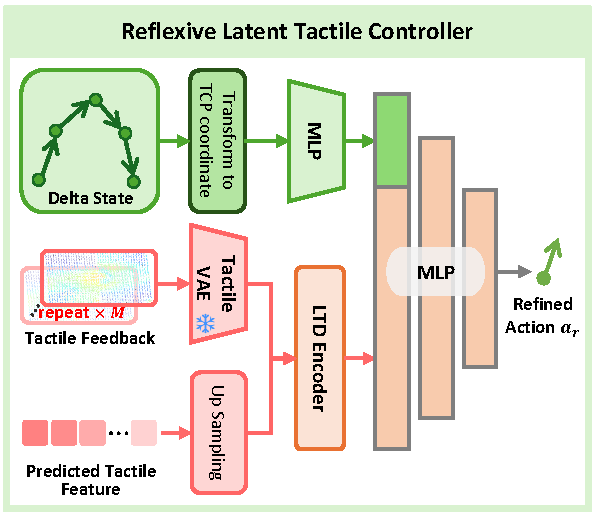
\includegraphics[width= 0.8\linewidth]{fig/controller.pdf}
\caption{\textbf{Overview of the Reflexive Latent Tactile Controller (RLTC).} It takes single-frame tactile feedback, predicted tactile latents, and robot/gripper delta states as input to produce high-frequency (60~Hz) refined single-step corrective actions.}
\label{fig:controller}
\end{figure}

\subsubsection{Training Loss}
To train the Reflexive Latent Tactile Controller, we learn corrective actions under abnormal contact conditions. For each task category, we first estimate a valid tactile distribution with its mean and standard deviation from human-collected trajectories. Tactile observations that fall outside this distribution (i.e., exhibiting excessively large or small contact forces) are identified as abnormal states.

We then extract recovery segments where the system transitions from abnormal tactile states back to the valid distribution, representing corrective behaviors demonstrated by human operators. 
For each time step in these segments, we construct training pairs consisting of the current tactile observation, the predicted tactile feature, and the corresponding corrective action $\hat{a}_r$.
The controller is trained to predict the corrective action $a_r$ using a mean squared error (MSE) loss:
\begin{equation}
\mathcal{L}_{RLTC} = \| a_r - \hat{a}_r \|_2^2,
\end{equation}
which encourages the controller to learn high-frequency tactile-driven corrections that stabilize contact interactions.

\section{Experimental Evaluation}
Our experiments are organized into three parts. First, we describe the experimental setup and implementation details. Second, we evaluate the overall performance of OmniVTA on manipulation tasks involving diverse tactile interaction patterns. Then, we conduct comprehensive ablation studies to analyze the contribution of each module in the proposed policy.
Specifically, we investigate the following questions: 
(1) whether the TactileVAE can effectively encode tactile signals; 
(2) whether the proposed visuo-tactile world model can predict future tactile signals more accurately than alternative tactile prediction approaches; 
(3) whether incorporating predicted future tactile signals improves policy performance and whether the proposed usage of predicted tactile information in OmniVTA is effective; and 
(4) whether the Reflexive Latent Tactile Controller can generate reasonable fine-grained corrective actions and how much it improves policy execution. 
We further analyze the contribution of each design component through detailed ablation studies.

\subsection{Experimental Setup}

\begin{table*}[t]
\centering
\caption{Objects used for training and manipulation across different robotic tasks. Each object is associated with 150 manipulation trajectories in the dataset for training world models and manipulation policies.}
\small
\renewcommand{\arraystretch}{1.2}
\begin{tabular}{@{} l l l @{}}
\toprule
\textbf{Task} & \textbf{Object Used for Training} & \textbf{Object Used for Manipulation} \\
\midrule
\textbf{Wipe} & vases in 4 different colors and shapes, plate, and whiteboard  & vases in 4 different colors and shapes \\
\textbf{Peel} & cucumber, Chinese yam, radish, carrot, and white daikon & cucumber, Chinese yam, radish \\
\textbf{Cut} & cucumber, Chinese yam, carrot, pepper, and banana & cucumber, Chinese yam, pepper, banana \\
\textbf{Assembly} & 3 colors of USB stick and 3 types of charging adapters & red USB stick and silver USB stick \\
\textbf{Grasp} & blueberry, strawberry, grape, cherry, and cherry tomato & blueberry, strawberry, grape, and cherry tomato \\
\textbf{Adjustment} & test tube, pencil, cuboid, cylinder, and triangular prism & cuboid, cylinder \\
\bottomrule
\label{tab:object}
\end{tabular}
\vspace{-5mm}
\end{table*}

\subsubsection{Training Details}
Our OmniVTA framework is trained in four stages: training the TactileVAE, training the Visuo-Tactile World Model, training the Adaptive Visuo-Tactile Fusion Policy, and training the Reflexive Latent Tactile Controller.

\noindent\textbf{Training of TactileVAE.}
For training the TactileVAE, we use tactile data from 20\% of the manipulation trajectories, together with additional tactile interaction data collected from interactions between 10 extra objects and the tactile sensors. The resulting dataset contains approximately 1.2M tactile samples. 
Both TactileVAE and the VAE baselines are trained for 50 epochs using 8 NVIDIA A100 GPUs.
The loss weights are set to $\lambda_{\text{KL}}=1e-6$.

\noindent\textbf{Training of Visuo-Tactile World Model.}
We first construct a dataset to train the Visuo-Tactile World Model, comprising six categories of tactile interaction patterns. 
For each category, 5--6 objects are selected, and 150 manipulation trajectories per object are collected using TacUMI and the xArm7. 
The data are split into training and test sets with a 90\%/10\% ratio. 
A detailed breakdown of the dataset is provided in Table~\ref{tab:object}.

For training the Visuo-Tactile World Model, we use AdamW with a learning rate of $1\times10^{-4}$ and weight decay $0$. The per-GPU batch size is $5$, and the total number of training steps is $100{,}000$. The gradient norm threshold is set to $0.1$, with gradient clipping enabled after $20{,}000$ steps. The loss weights are set to $\lambda_{\text{dyn}}=1.0$ and $\lambda_{\text{amp}}=1.0$.

\noindent\textbf{Training of Adaptive Visuo-Tactile Fusion Policy.}
We used the same training set to train the Adaptive Visuo-Tactile Fusion Policy.
For each interaction category, the data are combined to train a unified visuo-tactile generation and manipulation model (OmniVTA), as well as other policy baselines. 
The Adaptive Visuo-Tactile Fusion Policy is trained for 250k steps. Other manipulation baselines are trained for 350k steps to compensate for the absence of additional perception modules.
The loss weights are set to $\lambda_{ct}=0.2$.

\noindent\textbf{Parameter settings.}
Following prior work, we adopt \emph{relative actions} as the action representation. 
During training, visual observations are sampled at 15\,Hz, tactile signals at 60\,Hz, and robot proprioception at 60\,Hz. 
The policy outputs action chunks at 15\,FPS. 
For observations, both OmniVTA and all baselines use the current and previous visual frames (2 frames in total), the corresponding 8 tactile frames within the same temporal window, and 2 proprioceptive observations as policy inputs. 
Each action chunk predicts the next 6 actions, which are interpolated to 60\,Hz during execution.

\subsubsection{Hardware Setup}

The experimental platform consists of a UFactory xArm7 robotic arm equipped with a parallel two-finger gripper and two fingertip tactile sensors. 
An Intel RealSense D435 camera mounted on the robot wrist provides RGB observations at 15\,Hz, while the tactile sensors capture tactile signals at 60\,Hz. For the TactileVAE validation experiments, three types of tactile sensors are used: GelSight Mini, Tac3D, and Xense. 
The resolutions of their reconstructed 3D displacement fields are $7\times9$, $20\times20$, and $35\times20$, respectively. 
In the real-world manipulation experiments, we use only the Xense sensors.

\subsubsection{Baselines}
We select representative baseline methods to evaluate the effectiveness of the proposed TactileVAE, Visuo-Tactile World Model, and the overall OmniVTA framework. 

\noindent \textbf{TactileVAE baselines.} We compare the proposed TactileVAE with two representative tactile encoding methods: PCA-based features and a point cloud-based autoencoder~\cite{chen2024general}.

\noindent \textbf{Tactile prediction baselines.}
We compare our Visuo-Tactile World Model against three representative paradigms for multi-modal generative modeling.

\begin{itemize}
\item \textbf{Unified multimodal generation}:
UVA~\cite{li2025unified} models video frames and actions as a unified token sequence and jointly generates them using a single generative model. We extend this formulation by injecting tactile tokens.

\item \textbf{Joint trajectory diffusion}:
ForceMimic~\cite{liu2025forcemimic} and KineDex~\cite{zhang2025kinedex} concatenate interaction forces with actions and learn diffusion-based policies conditioned on visual observations. In our implementation, we replace force inputs with tactile feature embeddings extracted using a lightweight MLP autoencoder.

\item \textbf{Conditional modality prediction}:
exUMI~\cite{xu2025exumi} generates future tactile signals using a latent diffusion model (LDM) conditioned on visual observation and action. Since our method assumes only historical observations are available at inference, future action inputs are replaced with historical action sequences.
\end{itemize}

\noindent \textbf{Contact-rich policy baselines.}
We compare against several state-of-the-art imitation learning policies:

\begin{itemize}
\item \textbf{DP}~\cite{chi2025diffusion}: Diffusion Policy using wrist-view RGB observations and open-loop action chunk execution.
\item \textbf{DP+tactile}: Diffusion Policy augmented with tactile features encoded by PCA.
\item \textbf{KineDex}~\cite{zhang2025kinedex}: a diffusion policy that jointly predicts actions and forces from visual observations.
\item \textbf{ForceMimic}~\cite{liu2025forcemimic}: a diffusion policy conditioned on 3D observations that jointly predicts actions and forces.
\item \textbf{RDP}~\cite{xue2025reactive}: a reactive diffusion policy with a slow diffusion planner and a fast tactile-based reactive controller.
\item \textbf{OmniVTA (ours)}: our method with a visuo-tactile world model and a dual-system manipulation policy consisting of a diffusion planner and a reflexive tactile controller.
\item \textbf{OmniVTA w/o RLTC}: our method without the reflexive controller, executing diffusion-planned action chunks in a open-loop manner.
\end{itemize}

\begin{figure}[ht]
\centering
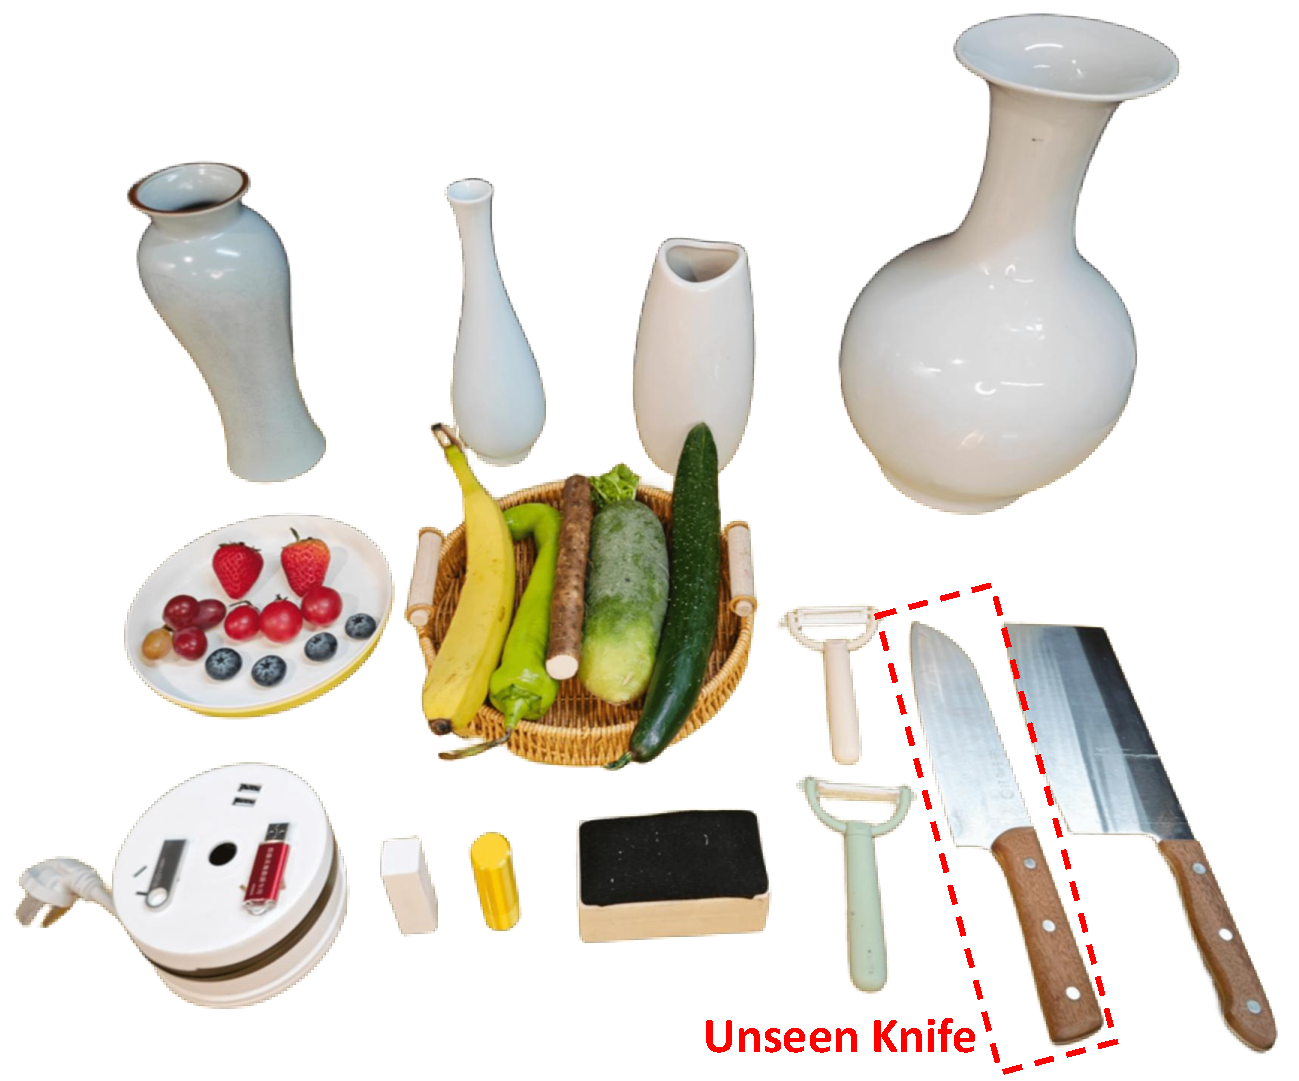
\includegraphics[width=0.75\linewidth]{fig/object.pdf}
\caption{\textbf{Objects used in the manipulation tasks.}}
\label{fig:object}
\vspace{-3mm}
\end{figure}

\subsection{Overall Performance}

We evaluate the real-world manipulation performance of OmniVTA from three perspectives: object diversity, generalization, and perturbation robustness.

\noindent \textbf{Object diversity.}
For each category, we evaluate the policy on 2--4 different objects, as summarized in Table~\ref{tab:object} and Fig.~\ref{fig:object}. 
Before each trial, the object is placed at a random position and fixed during manipulation. 
For each object, we perform 10 trials and report the average success rate.

\noindent \textbf{Generalization.}
We evaluate two types of generalization.

(1) \emph{Position generalization.}
For the wipe, peel, assembly, and adjustment tasks, objects are placed at two additional unseen heights during evaluation. 
For each object and each height, we conduct 5 trials and report the average success rate.

(2) \emph{Tool generalization.}
For the cut task, we replace the training knife with a previously unseen knife (shown in Fig.~\ref{fig:object}). 
Each object is tested 10 times using the new tool.


\noindent \textbf{Perturbation robustness.}
For the wipe, peel, cut, and assembly tasks, we introduce controlled perturbations during execution to disrupt the current contact state. 
Specifically, the target object is suddenly displaced upward or downward along the vertical direction during the interaction phase. 
This perturbation breaks the existing contact state and requires the policy to re-establish stable contact. 
For each task, one representative object is selected and evaluated over 10 trials.

\noindent \textbf{Evaluation metric.}
The primary evaluation metric is task success rate. 
A trial is considered successful if the task objective is completed and no damage occurs to the tactile sensors during execution. For wiping, peeling, and cutting tasks, we measure task completion using the ratio of the successfully processed length (e.g., the proportion of removed peel, erased marks, or completed cuts). For assembly and grasping tasks, a trial is considered successful only if the object is fully inserted or grasped without damage. For adjustment tasks, success is defined as achieving a pose change that exceeds a predefined angular threshold (60°).

\noindent \textbf{Results.}
The overall real-robot manipulation results are visualized in Fig.~\ref{fig:manipulation}, and the corresponding overall success rates are reported in Table~\ref{tab:full_comparison_final_scaled}.
In the object diversity evaluation, OmniVTA achieves the best performance across all six tasks, demonstrating the effectiveness of the proposed framework. 
Adding the closed-loop controller further improves performance compared with the open-loop variant (OmniVTA w/o RLTC), highlighting the importance of feedback control in contact-rich manipulation.

\begin{figure*}[t]
\centering
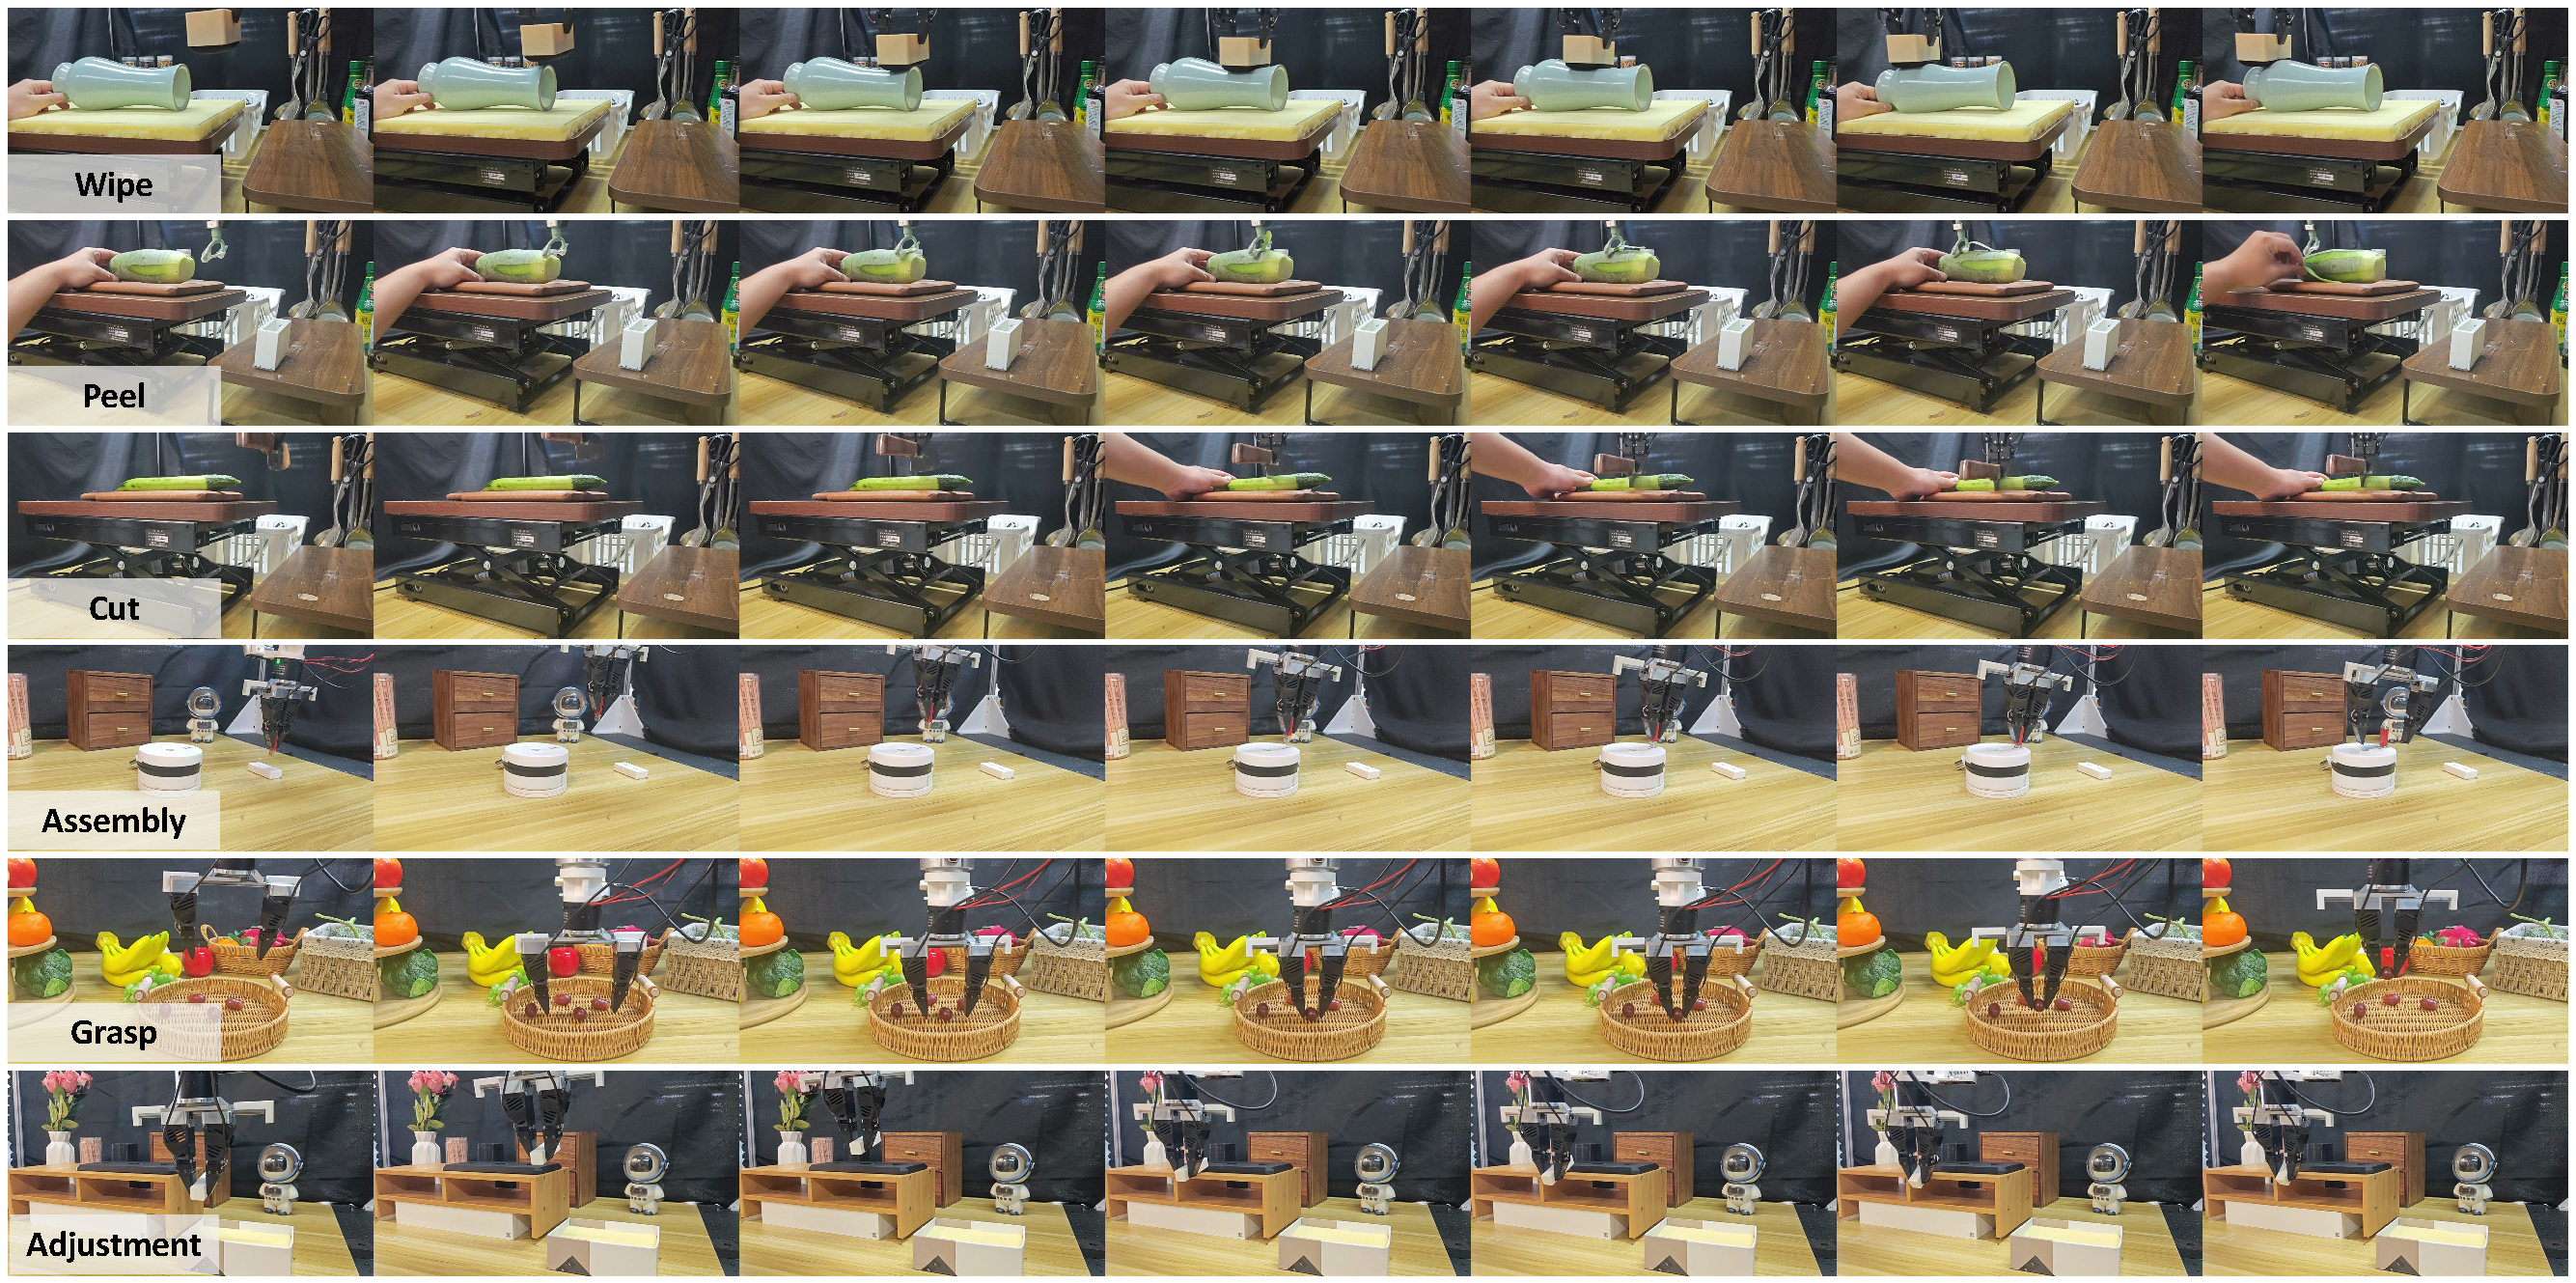
\includegraphics[width=0.95\linewidth]{fig/manipulation.pdf}
\caption{\textbf{Real-robot manipulation results.} We visualize the manipulation process across six task categories.}
\label{fig:manipulation}
\end{figure*}

\begin{table*}[t]
\centering
\caption{Performance comparison of OmniVTA and baseline methods across six tasks under three evaluation settings: object diversity (O), generalization (G), and perturbation robustness (P). Results are reported in terms of success rate.}
\label{tab:full_comparison_final_scaled}
\small
\setlength{\tabcolsep}{2.5pt}
\renewcommand{\arraystretch}{1.3}

\begin{tabularx}{\textwidth}{@{} l *{15}{>{\centering\arraybackslash}X} @{}}
\toprule
\textbf{Task} & \multicolumn{3}{c}{\textbf{Wipe}} & \multicolumn{3}{c}{\textbf{Peel}} & \multicolumn{3}{c}{\textbf{Cut}} & \multicolumn{3}{c}{\textbf{Assembly}} & \multicolumn{1}{c}{\textbf{Grasp}} & \multicolumn{2}{c}{\textbf{Adjustment}} \\
\cmidrule(lr){2-4} \cmidrule(lr){5-7} \cmidrule(lr){8-10} \cmidrule(lr){11-13} \cmidrule(lr){14-14} \cmidrule(lr){15-16}
\makecell[l]{\textbf{Method /}\textbf{ Eval. setting}} & \textbf{O} & \makecell[c]{{\textbf{G}}} & \textbf{P} & \textbf{O} & \makecell[c]{\textbf{G}} & \textbf{P} & \textbf{O} & \makecell[c]{{\textbf{G}}} & \textbf{P} & \textbf{O} & \makecell[c]{{\textbf{G}}} & \textbf{P} & \textbf{O} & \textbf{O} & \makecell[c]{\textbf{G}} \\
\midrule
DP               & 0.12 & 0.05 & 0 & 0.06 & 0 & 0 & 0.28 & 0.10 & 0 & 0.10 & 0 & 0.05 & 0.20 & 0 & 0 \\
DP+tactile       & 0.36 & 0.28 & 0 & 0.32 & 0.20 & 0.08 & 0.33 & 0.15 & 0.13 & 0.30 & 0.10 & 0.10 & 0.48 & 0.25 & 0.15 \\
KineDex          & 0.40 & 0.25 & 0 & 0.24 & 0.13 & 0.05 & 0.38 & 0.30 & 0.20 & 0.30 & 0.15 & 0.15 & 0.65 & 0.30 & 0.20 \\
ForceMimic       & 0.33 & 0.20 & 0 & 0.27 & 0.18 & 0 & 0.50 & 0.25 & 0.05 & 0.35 & 0.15 & 0.10 & 0.60 & 0.10 & 0 \\
RDP              & 0.50 & 0.38 & 0.42 & 0.48 & 0.36 & 0.45 & 0.65 & 0.50 & 0.43 & \textbf{0.60} & \textbf{0.50} & 0.35 & 0.88 & 0.50 & 0.50 \\
OmniVTA w/o RLTC & 0.66 & 0.40 & 0.25 & 0.40 & 0.30 & 0.20 & 0.50 & 0.50 & 0.20 & 0.40 & 0.35 & 0.20 & 0.70 & 0.40 & 0.30 \\
\textbf{OmniVTA} & \textbf{0.80} & \textbf{0.58} & \textbf{0.60} & \textbf{0.55} & \textbf{0.48} & \textbf{0.63} & \textbf{0.85} & \textbf{0.83} & \textbf{0.60} & \textbf{0.60} & \textbf{0.50} & \textbf{0.40} & \textbf{0.90} & \textbf{0.65} & \textbf{0.65} \\
\bottomrule
\end{tabularx}
\vspace{-3mm}
\end{table*}

We also observe that, for contact-rich tasks involving strong physical interactions (e.g., wiping, peeling, cutting), the performance gain from the reactive policy in RDP (compared with DP+tactile) is smaller than the improvement brought by our reflexive controller.
This is because our controller leverages predicted tactile signals as targets to regulate the robot's motion, enabling reliable contact while preventing excessive contact forces. 
During the contact phase, the average tangential deformation measured by our tactile sensors is 0.35 with a maximum of 0.72. 
In contrast, the reactive policy in RDP often produces overly strong contacts that damage the sensors, with an average deformation of 0.56 and a maximum of 1.1. In the unseen-height evaluation, the performance of RDP drops moderately, while other baselines degrade significantly. 
In contrast, OmniVTA without the closed-loop controller already surpasses RDP, indicating stronger robustness to geometric variations. In the tool generalization experiment, replacing the knife with a smaller, unseen tool has little impact on our performance in the cut task. 
This suggests that the policy relies on tactile feedback rather than memorizing demonstration trajectories. Finally, in the perturbation experiments, OmniVTA consistently achieves the highest success rates. 
Moreover, the closed-loop controller significantly improves performance compared with the open-loop variant, demonstrating its ability to quickly recover stable contact during perturbations.

\vspace{-3mm}
\subsection{Component Analysis}
\subsubsection{TactileVAE}
We evaluate TactileVAE from two aspects: reconstruction accuracy and latent representation quality.

\noindent \textbf{Reconstruction evaluation.}
We compare TactileVAE with baseline methods across six categories of tactile interaction patterns. 
Reconstruction performance is evaluated using the $L_2$ distance and cosine similarity, which measure the magnitude and directional consistency of the reconstructed 3D deformation, respectively. 
The $L_2$ metric is computed over the entire deformation field, while cosine similarity is computed over non-zero deformation regions only. 
As shown in Table~\ref{tab:vae}, the proposed TactileVAE consistently achieves the best performance across all six categories, demonstrating its effectiveness in modeling tactile deformation.

\begin{table*}[t]
\centering
\caption{Performance comparison of different methods across robotic tasks using L2 and cosine similarity metrics. Lower L2 ($\downarrow$) and higher cos ($\uparrow$) indicate better performance.}
\label{tab:vae}
\small 
\renewcommand{\arraystretch}{1.2}

\begin{tabular*}{\textwidth}{@{\extracolsep{\fill}} l ccccc ccccc cc}
\toprule
\textbf{Method} & \multicolumn{2}{c}{\textbf{Wipe}} & \multicolumn{2}{c}{\textbf{Peel}} & \multicolumn{2}{c}{\textbf{Cut}} & \multicolumn{2}{c}{\textbf{Assembly}} & \multicolumn{2}{c}{\textbf{Grasp}} & \multicolumn{2}{c}{\textbf{Adjustment}} \\
\cmidrule(lr){2-3} \cmidrule(lr){4-5} \cmidrule(lr){6-7} \cmidrule(lr){8-9} \cmidrule(lr){10-11} \cmidrule(lr){12-13}
& {L2 $\downarrow$} & {cos $\uparrow$} & {L2 $\downarrow$} & {cos $\uparrow$} & {L2 $\downarrow$} & {cos $\uparrow$} & {L2 $\downarrow$} & {cos $\uparrow$} & {L2 $\downarrow$} & {cos $\uparrow$} & {L2 $\downarrow$} & {cos $\uparrow$} \\
\midrule
PCA         & 0.091 & 0.810 & 0.085 & 0.430 & 0.109 & 0.400 & 0.071 & 0.720 & 0.036 & 0.600 & 0.069 & 0.560 \\
PointNet-AE & 0.059 & 0.910 & 0.067 & 0.850 & 0.062 & 0.840 & 0.058 & 0.900 & 0.028 & \textbf{0.750} & 0.047 & 0.760 \\
\textbf{Ours} & \textbf{0.038} & \textbf{0.930} & \textbf{0.033} & \textbf{0.880} & \textbf{0.031} & \textbf{0.940} & \textbf{0.022} & \textbf{0.910} & \textbf{0.011} & 0.720 & \textbf{0.017} & \textbf{0.850} \\
\bottomrule
\end{tabular*}
\end{table*}

\noindent \textbf{Latent representation analysis.}
To further evaluate the learned tactile representations, we conduct experiments on three unseen objects under three types of force patterns (press, twist, and slide) using three tactile sensors, two of which are unseen during training, as shown in Fig.~\ref{fig:vae_tsne}(a) and (b). 
We record the tactile signals and extract their features using several variants of TactileVAE, including:
\begin{itemize}
    \item \textbf{w/o implicit decoder:} decodes the latent feature map without query-based sampling and query points input.
    \item \textbf{w/ position embedding:} incorporates positional encoding during decoding.
    \item \textbf{w/o spatial feature map:} represents the latent as a single token and decodes it with an implicit decoder.
    \item \textbf{w/ implicit decoder:} decodes the latent feature map via an implicit decoder.
\end{itemize}
All models are trained using only 5\% of the tactile dataset.

For visualization, the spatio-temporal tactile features are aggregated via max pooling to obtain sequence-level embeddings, which are then visualized using t-SNE. 
As shown in Fig.~\ref{fig:vae_tsne}(c), the learned representations exhibit clear clustering across different force patterns, even under cross-sensor settings. 
In contrast, marker-based encoding and variants without positional information fail to produce well-separated clusters, highlighting the importance of implicit neural representations for learning discriminative tactile features.

Finally, we compare two forms of tactile feature representations: local feature maps (patch-based features) and a global token obtained via max pooling. 
As shown in Fig.~\ref{fig:vae_tsne}(c) and Table~\ref{tab:vae_ablation}, local feature maps achieve better reconstruction accuracy and yield more informative tactile embeddings than the global token representation.

\begin{table}[t]
\centering
\caption{Ablation study on the design of TactileVAE. We evaluate reconstruction performance using the $L_2$ metric.}
\label{tab:vae_ablation}
\small
\renewcommand{\arraystretch}{1.2} % 增加行间距，提升阅读舒适度
% 设置列间距，让1栏宽度的表格看起来更紧凑
\setlength{\tabcolsep}{2pt} 

\begin{tabular}{l S[table-format=1.3] S[table-format=1.3] S[table-format=1.3]}
\toprule
\textbf{Method} & {\textbf{GelSight-Mini}} & {\textbf{Tac3D-A1}} & {\textbf{Xense-QN1}} \\
\midrule
w/o implicit decoder & 0.126 & 0.098 & 0.038 \\
w/ position embed. & 0.102 & 0.085 & 0.035 \\
w/o spatial feature map & 0.107 & 0.084 & 0.071 \\
w/ implicit decoder & \textbf{0.047} & \textbf{0.058} & \textbf{0.034} \\
\bottomrule
\end{tabular}
\end{table}

\begin{figure}[ht]
\centering
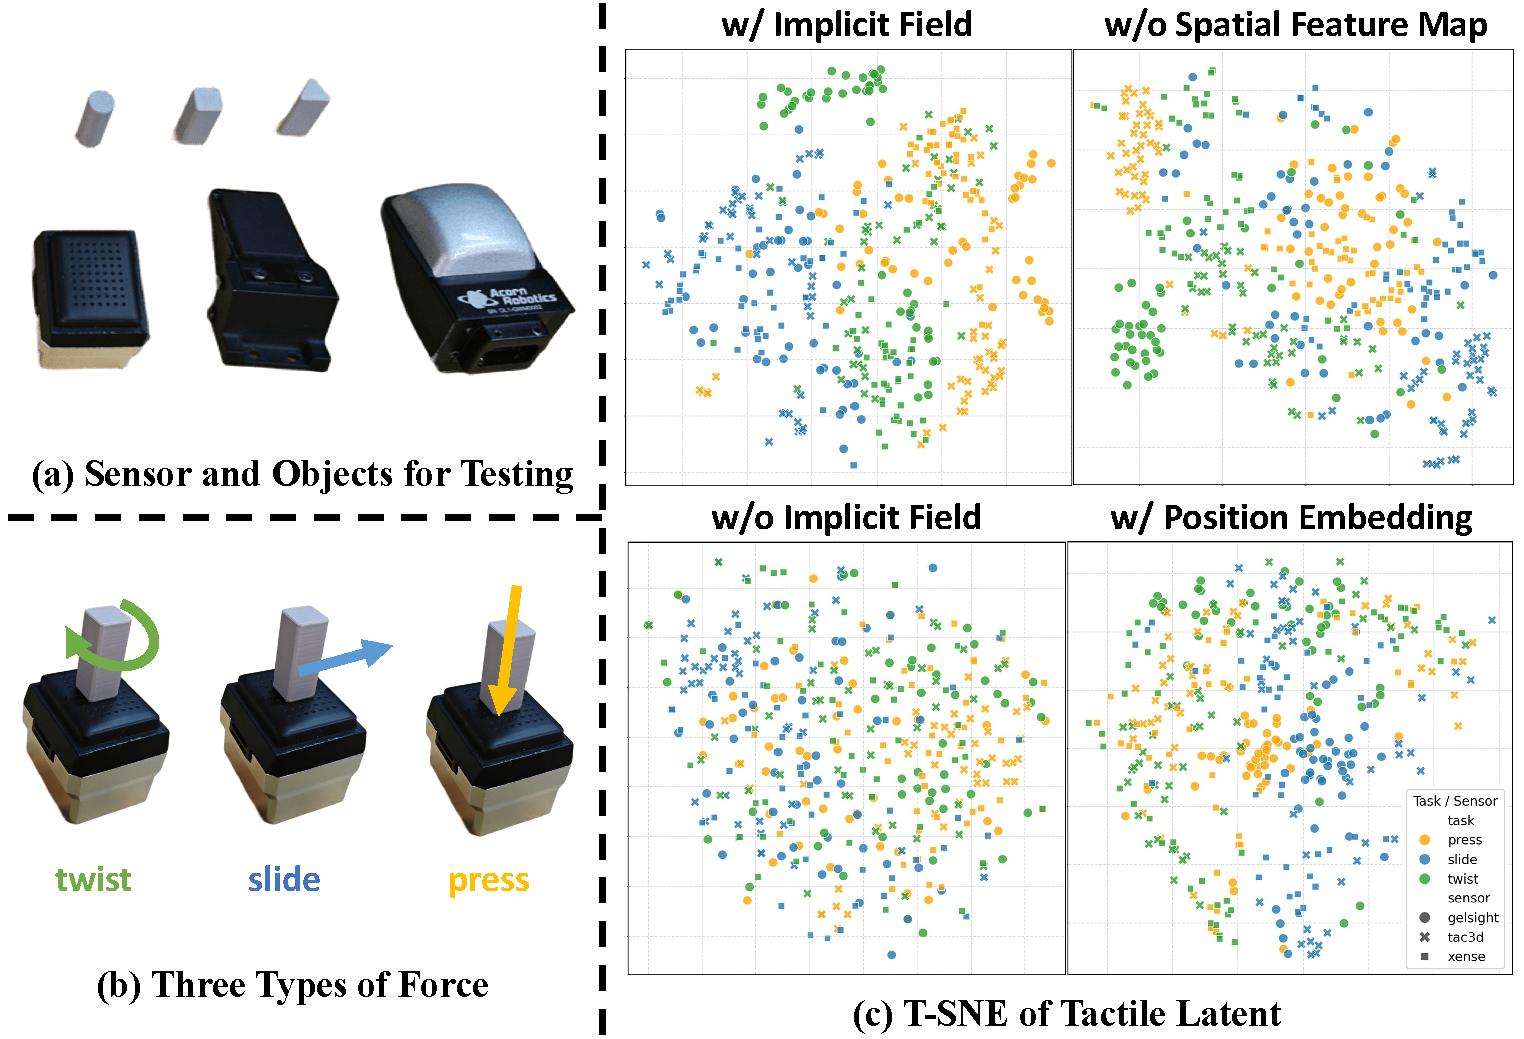
\includegraphics[width=\linewidth]{fig/tsne.pdf}
\caption{\textbf{Ablation study of TactileVAE.}\textbf{(a)} shows the sensors and objects for testing. \textbf{(b)} represents the three types of force loaded on the sensors. \textbf{(c)} visualizes the t-SNE of the tactile latent feature maps extracted by different models.}
\label{fig:vae_tsne}
\vspace{-3mm}
\end{figure}

\subsubsection{Visuo-Tactile World Model}

\begin{figure*}[ht]
\centering
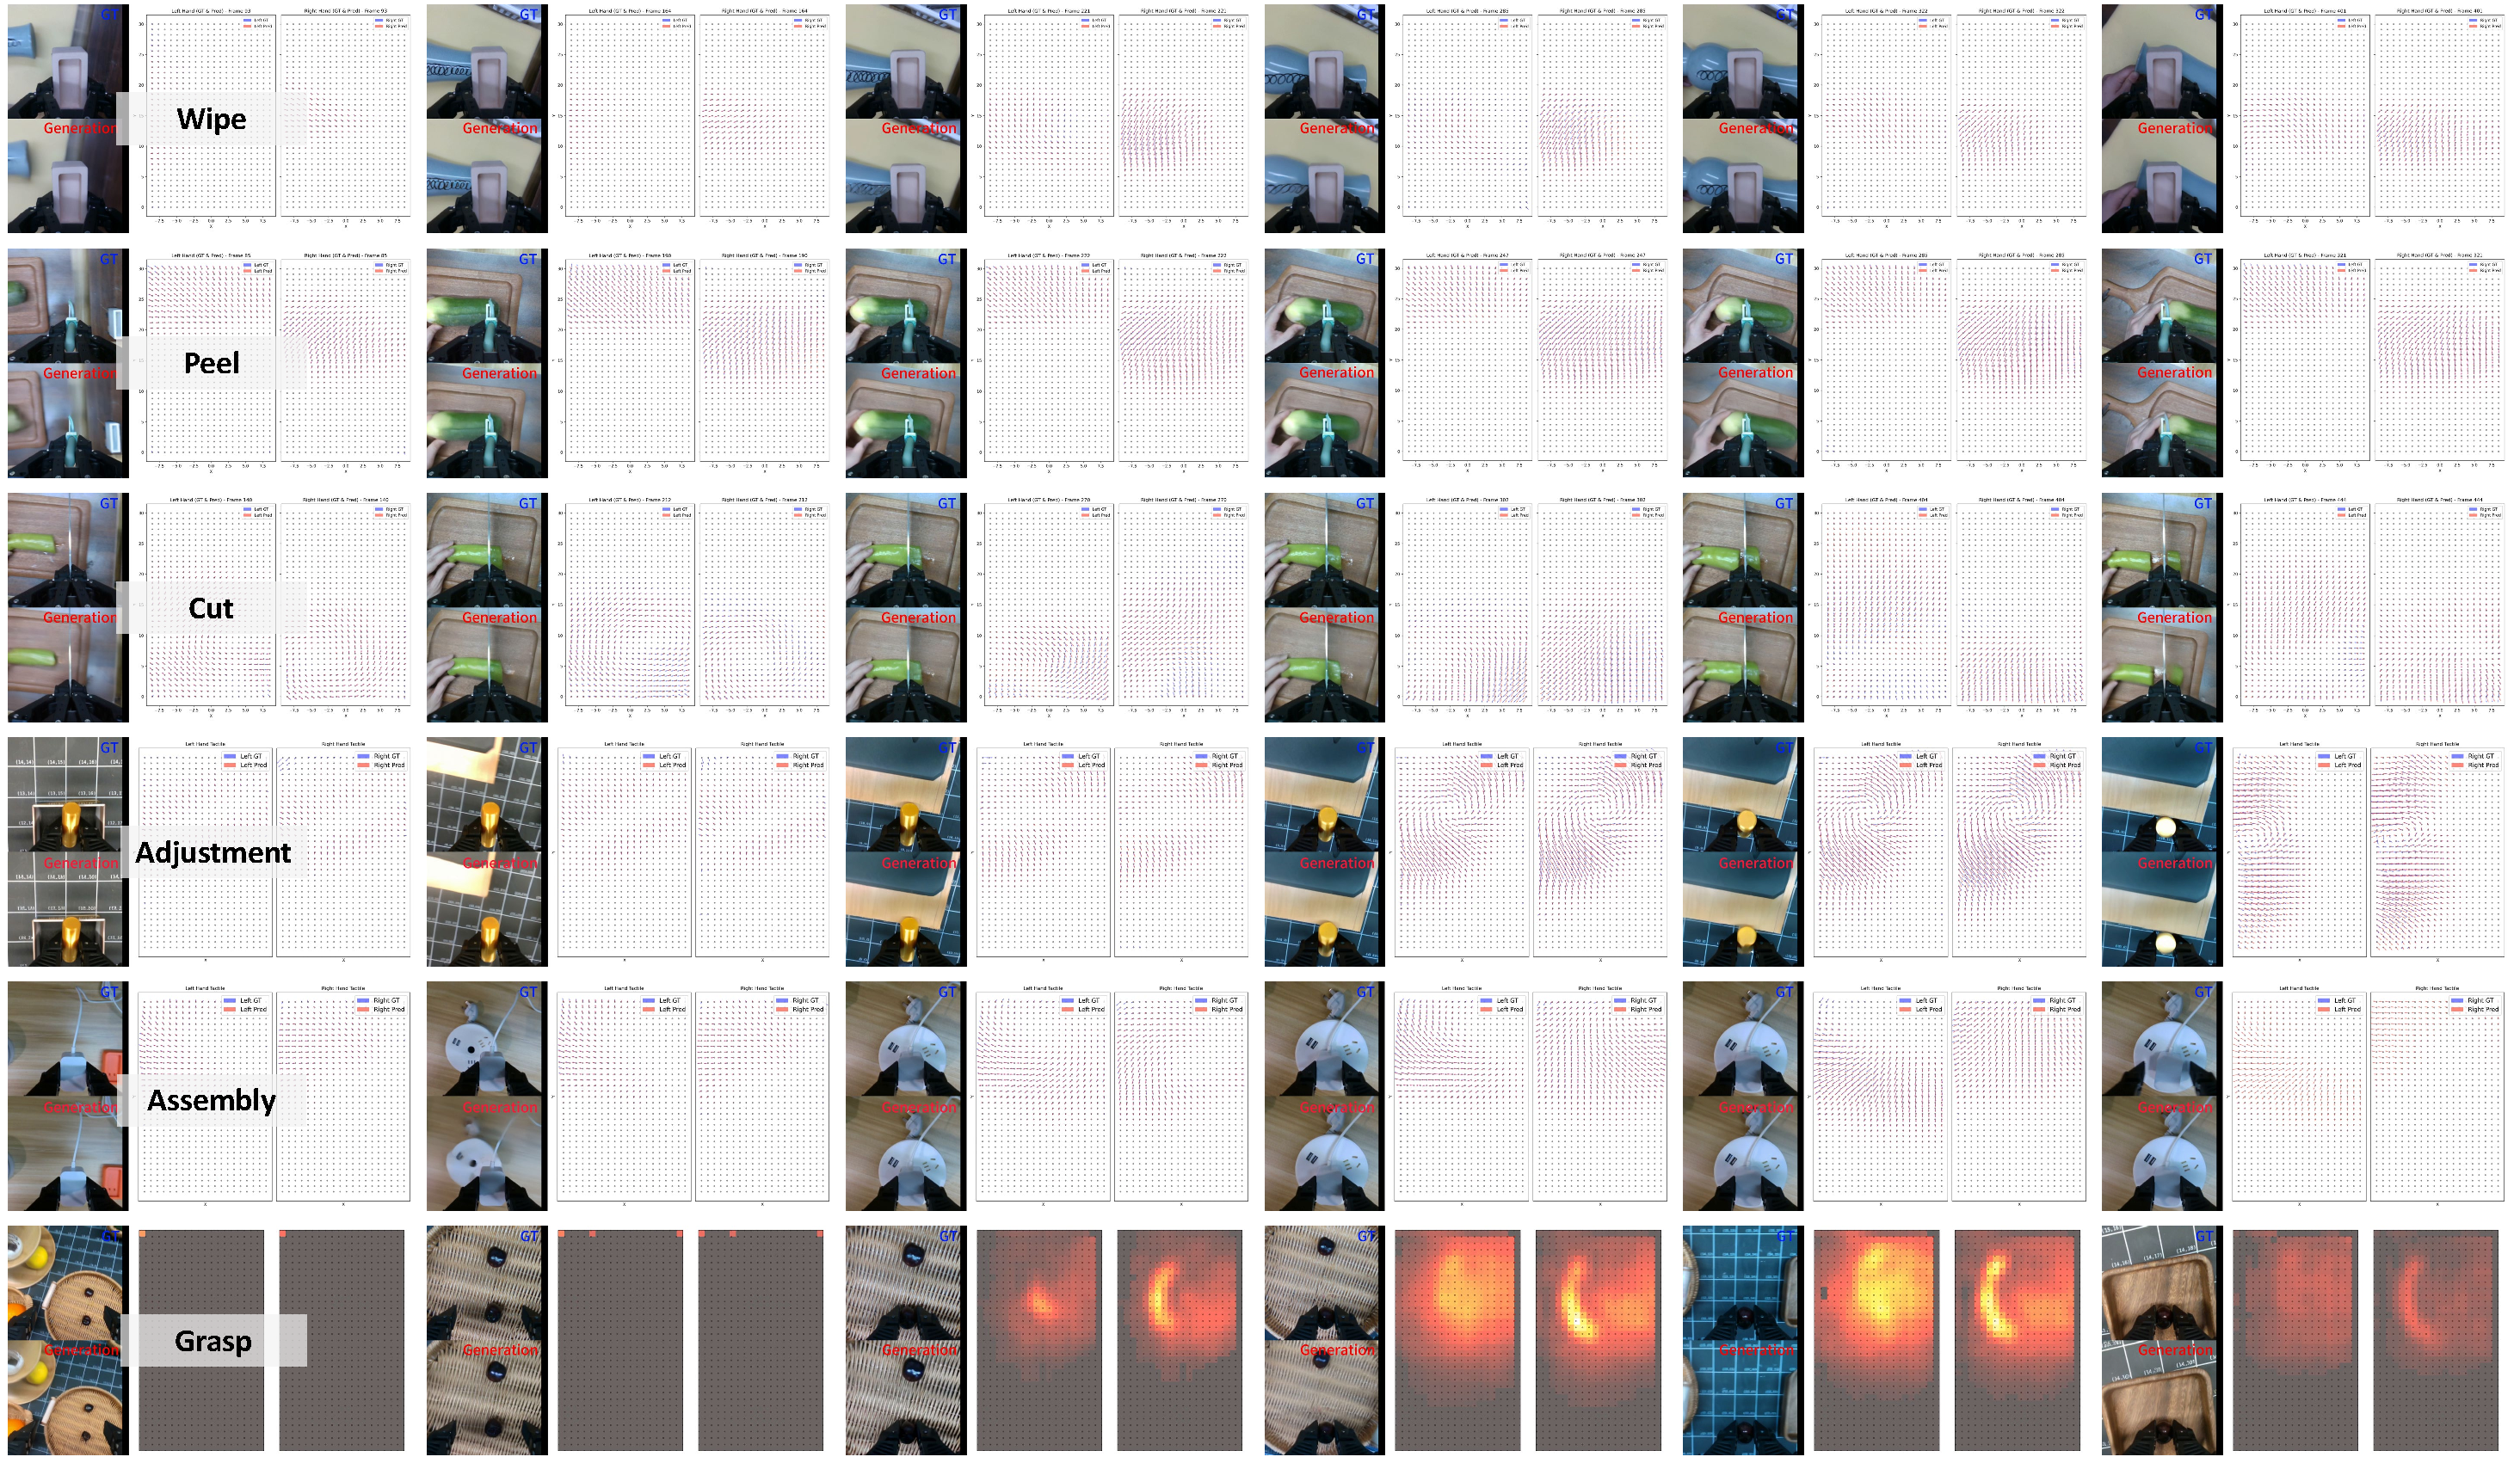
\includegraphics[width=\linewidth]{fig/wm.pdf}
\caption{\textbf{Visuo-tactile generation visualization across six task categories.} Red arrows indicate predicted tangential deformation, while blue arrows denote ground truth. Normal deformation in the grasp task is visualized using heatmaps. }
\label{fig:wm}
\end{figure*}

% 需要的宏包（如果你还没引入）：
% \usepackage{graphicx}   % for \resizebox
% \usepackage{multirow}   % 可选
% \usepackage{amsmath}    % 可选（数学下标更舒服）

% =========================
% Row 1: wipe / peel / cut
% =========================
\begin{table*}[t]
\centering
\scriptsize
\setlength{\tabcolsep}{2pt}
\renewcommand{\arraystretch}{1.15}
\caption{Prediction performance. We report the $L_2$ distance and cosine similarity at the 2nd, 4th, and 6th latent prediction steps (denoted as $L2_1, L2_2, L2_3$ and $C_1, C_2, C_3$), corresponding to the 8th, 16th, and 24th decoded tactile frames, respectively. We also report the average performance over all 24 predicted frames ($L2_{\text{avg}}$, $C_{\text{avg}}$). Top: Wipe/Peel/Cut. Bottom: Adjustment/Assembly/Grasp. ``--" denotes not applicable.}
\label{tab:wm_exp}
\resizebox{\textwidth}{!}{%
\begin{tabular}{l|cccccccc|cccccccc|cccccccc}
\hline
\multicolumn{1}{c|}{} &
\multicolumn{8}{c|}{\textbf{Wipe}} &
\multicolumn{8}{c|}{\textbf{Peel}} &
\multicolumn{8}{c}{\textbf{Cut}} \\
\hline
\textbf{Method} &
$L2_1$ & $L2_2$ & $L2_3$ & $L2_{\text{avg}}$ & $C_1$ & $C_2$ & $C_3$ & $C_{\text{avg}}$ &
$L2_1$ & $L2_2$ & $L2_3$ & $L2_{\text{avg}}$ & $C_1$ & $C_2$ & $C_3$ & $C_{\text{avg}}$ &
$L2_1$ & $L2_2$ & $L2_3$ & $L2_{\text{avg}}$ & $C_1$ & $C_2$ & $C_3$ & $C_{\text{avg}}$ \\
\hline
\textbf{UVA} &
0.084 & 0.091 & 0.088 & 0.088 & 0.68 & 0.65 & 0.64 & 0.66 &
0.090 & 0.097 & 0.102 & 0.097 & 0.62 & 0.60 & 0.60 & 0.61 &
0.075 & 0.076 & 0.078 & 0.077 & 0.72 & 0.71 & 0.71 & 0.71 \\

\textbf{exUMI} &
0.097 & 0.098 & 0.103 & 0.101 & 0.59 & 0.58 & 0.58 & 0.58 &
0.093 & 0.099 & 0.102 & 0.097 & 0.63 & 0.62 & 0.62 & 0.62 &
0.083 & 0.086 & 0.088 & 0.086 & 0.73 & 0.72 & 0.71 & 0.72 \\

\textbf{Kinedex} &
0.081 & 0.084 & 0.085 & 0.082 & 0.82 & 0.80 & 0.81 & 0.81 &
0.064 & 0.066 & 0.068 & 0.066 & 0.77 & 0.79 & 0.80 & 0.79 &
0.091 & 0.100 & 0.104 & 0.096 & 0.74 & 0.73 & 0.72 & 0.73 \\

\textbf{Forcemimic} &
0.089 & 0.091 & 0.094 & 0.091 & 0.70 & 0.68 & 0.68 & 0.68 &
0.077 & 0.077 & 0.078 & 0.077 & 0.76 & 0.76 & 0.73 & 0.76 &
0.089 & 0.091 & 0.091 & 0.090 & 0.71 & 0.71 & 0.72 & 0.71 \\

\textbf{Ours} &
\textbf{0.052} & \textbf{0.062} & \textbf{0.072} & \textbf{0.059} & \textbf{0.93} & \textbf{0.92} & \textbf{0.91} & \textbf{0.93} &
\textbf{0.033} & \textbf{0.037} & \textbf{0.041} & \textbf{0.036} & \textbf{0.88} & \textbf{0.88} & \textbf{0.87} & \textbf{0.87} &
\textbf{0.048} & \textbf{0.052} & \textbf{0.057} & \textbf{0.050} & \textbf{0.89} & \textbf{0.89} & \textbf{0.88} & \textbf{0.88} \\
\hline
% \multicolumn{25}{c}{} \\
\hline
\multicolumn{1}{c|}{} &
\multicolumn{8}{c|}{\textbf{Adjustment}} &
\multicolumn{8}{c|}{\textbf{Assembly}} &
\multicolumn{8}{c}{\textbf{Grasp}} \\
\hline
\textbf{Method} &
$L2_1$ & $L2_2$ & $L2_3$ & $L2_{\text{avg}}$ & $C_1$ & $C_2$ & $C_3$ & $C_{\text{avg}}$ &
$L2_1$ & $L2_2$ & $L2_3$ & $L2_{\text{avg}}$ & $C_1$ & $C_2$ & $C_3$ & $C_{\text{avg}}$ &
$L2_1$ & $L2_2$ & $L2_3$ & $L2_{\text{avg}}$ & $C_1$ & $C_2$ & $C_3$ & $C_{\text{avg}}$ \\
\hline
\textbf{UVA} &
0.080 & 0.085 & 0.084 & 0.083 & 0.73 & 0.68 & 0.67 & 0.69 &
0.072 & 0.074 & 0.078 & 0.074 & 0.74 & 0.69 & 0.68 & 0.68 &
0.079 & 0.080 & 0.085 & 0.080 & 0.67 & 0.64 & 0.64 & 0.65 \\

\textbf{exUMI} &
0.080 & 0.087 & 0.083 & 0.083 & 0.64 & 0.60 & 0.60 & 0.61 &
0.096 & 0.096 & 0.103 & 0.096 & 0.59 & 0.53 & 0.52 & 0.53 &
0.076 & 0.081 & 0.085 & 0.081 & 0.66 & 0.65 & 0.63 & 0.65 \\

\textbf{Kinedex} &
0.052 & 0.053 & 0.055 & 0.053 & 0.70 & 0.70 & 0.69 & 0.70 &
0.045 & 0.048 & 0.052 & 0.047 & 0.80 & 0.77 & 0.75 & 0.78 &
0.017 & 0.017 & 0.017 & 0.017 & 0.60 & 0.60 & 0.58 & 0.59 \\

\textbf{Forcemimic} &
0.082 & 0.081 & 0.082 & 0.082 & 0.66 & 0.65 & 0.65 & 0.65 &
0.071 & 0.071 & 0.071 & 0.071 & 0.69 & 0.68 & 0.67 & 0.68 &
-- & -- & -- & -- & -- & -- & -- & -- \\

\textbf{Ours} &
\textbf{0.022} & \textbf{0.025} & \textbf{0.028} & \textbf{0.025} & \textbf{0.85} & \textbf{0.84} & \textbf{0.84} & \textbf{0.85} &
\textbf{0.028} & \textbf{0.032} & \textbf{0.036} & \textbf{0.030} & \textbf{0.90} & \textbf{0.89} & \textbf{0.88} & \textbf{0.89} &
\textbf{0.010} & \textbf{0.010} & \textbf{0.010} & \textbf{0.010} & \textbf{0.70} & \textbf{0.67} & \textbf{0.67} & \textbf{0.68} \\
\hline
\end{tabular}}%
\end{table*}

\begin{table}[t]
\centering
\caption{Performance evaluation under different test cases, action spaces, and dynamic weight settings. Lower $L_2$ and higher cosines indicate better performance.}
\label{tab:ablation_wm}
\small
\setlength{\tabcolsep}{4pt}
\renewcommand{\arraystretch}{1.2} % 稍微加高，让多行合并的单元格不显得拥挤

\begin{tabular}{lccccc}
\toprule
\textbf{Settings} & \textbf{Action} & \textbf{Dyn. Weight} & \textbf{Joint Gen.} & \textbf{L2} $\downarrow$ & \textbf{Cos} $\uparrow$ \\
\midrule
\multirow{3}{*}{\makecell[c]{Unseen\\Position}} 
    & 3D absolute & \checkmark & \checkmark & 0.075 & 0.72 \\
    & 3D relative & \checkmark & \checkmark & 0.056 & 0.88 \\
    & 2D          & \checkmark & \checkmark & \textbf{0.042} & \textbf{0.91} \\
\midrule
\multirow{3}{*}{\makecell[c]{Seen\\Position}} 
    & 2D          & $\times$ & $\times$ & 0.041 & 0.90 \\
    & 2D          & $\times$ & \checkmark & 0.038 & 0.92 \\
    & 2D          & \checkmark & \checkmark & \textbf{0.035} & \textbf{0.93} \\
\bottomrule
\end{tabular}
\end{table}

In this section, we evaluate the proposed Visuo-Tactile World Model in terms of prediction accuracy, module effectiveness, and robustness to observation perturbations.
We measure tactile prediction accuracy using the $L_2$ distance and cosine similarity between the predicted and ground-truth tactile signals, following the evaluation
protocol of TactileVAE.
To better illustrate prediction performance over different horizons, we report both the $L_2$ distance and cosine similarity at the 2nd, 4th, and 6th prediction latent frames,
corresponding to the 8th, 16th, and 24th decoded tactile frames, respectively, as well as the metrics averaged over all 24 predicted frames.


% measuring magnitude accuracy and directional consistency of the predicted deformation, respectively. The $L_2$ metric is computed over the full deformation field, while cosine similarity is computed on flattened deformation vectors. All metrics are averaged over all time steps and trajectories.

\noindent \textbf{Prediction accuracy.}
We first compare our method with four baselines from three representative paradigms: unified multimodal generation, joint trajectory diffusion, and conditional tactile prediction. 
As shown in Table~\ref{tab:wm_exp} and Fig.~\ref{fig:wm}, our model consistently outperforms all baselines in both short-term and long-term tactile prediction. These results demonstrate that our method effectively models the cross-modal dynamics between vision and tactile signals, enabling accurate and consistent generation across both modalities.

\noindent \textbf{Ablation study.}
We further analyze the contribution of several key components in the proposed model.

(1) \emph{Joint visual–tactile generation.} 
Table~\ref{tab:ablation_wm} shows that jointly generating future visual features together with tactile features improves tactile prediction accuracy. 
This indicates that visual prediction provides complementary global dynamic cues that help the model better capture interaction dynamics.

(2) \emph{Action representation.}
We compare three types of action conditioning in the world model: projected 2D actions, 3D absolute actions, and 3D relative actions. 
As shown in Table~\ref{tab:ablation_wm}, the 2D action representation achieves the best generalization performance on unseen object positions, followed by relative actions. 
This result suggests that the action condition primarily conveys motion intent and that 2D actions align more naturally with visual observations.

(3) \emph{Dynamic weighting.}
The results in Table~\ref{tab:ablation_wm} show that the proposed dynamic weighting strategy improves tactile prediction performance. 
This weighting mechanism explicitly emphasizes regions with rapid dynamics and strong contact responses during optimization, enabling the model to better capture high-frequency tactile patterns, local contact variations, and fine-grained temporal structures.

\noindent \textbf{Perturbation robustness.}
Finally, we evaluate the robustness of the Visuo-Tactile World Model in the wipe-vase task. 
After contact occurs, the visual and tactile observations are replaced with non-contact observations corresponding to the object being moved downward. 
As shown in Fig.~\ref{fig:wm_disturb}, the model exhibits a certain level of recovery capability under observation perturbations.

\begin{figure*}[ht]
\centering
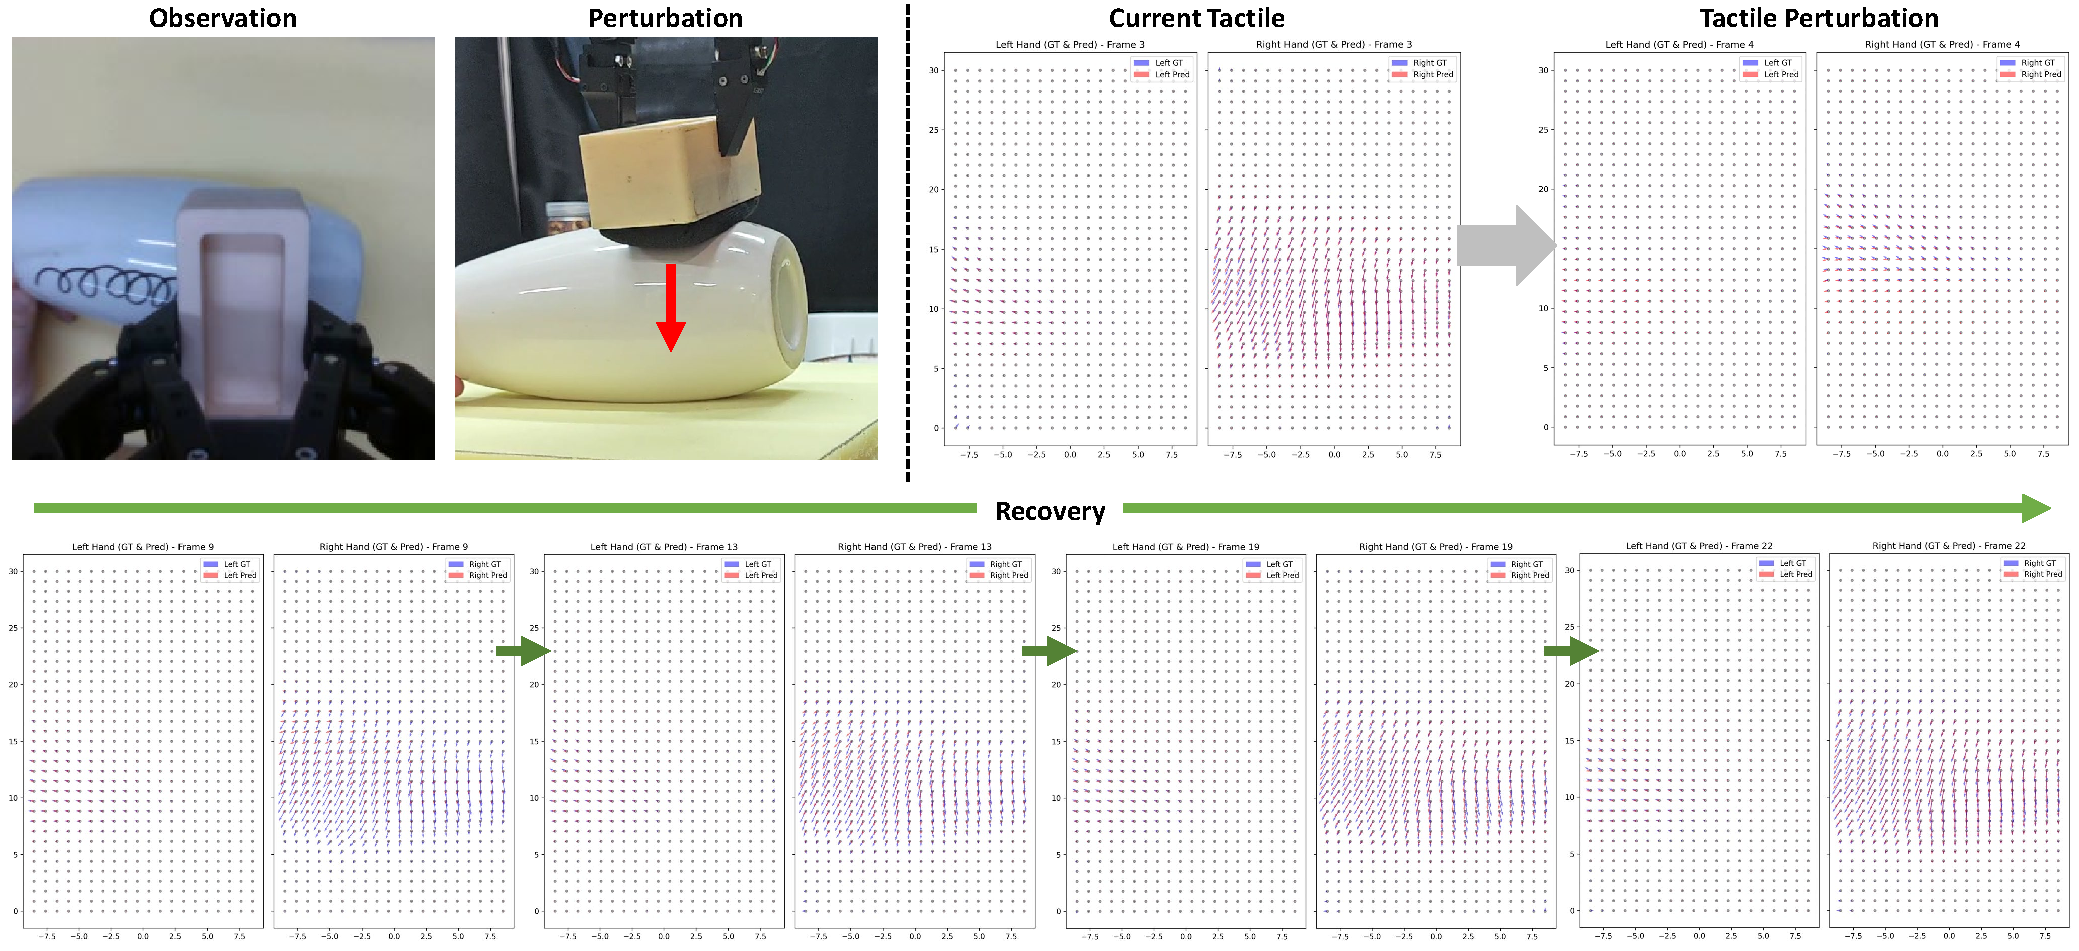
\includegraphics[width=0.95\linewidth]{fig/wm_disturb.pdf}
\caption{\textbf{Perturbation and recovery.} The first row shows a contact break due to downward perturbation, with tactile signals transitioning to a no-contact state. The second row shows recovery to the contact state within one generation chunk. In tactile visualization, red arrows denote tactile prediction while blue arrows denote ground truth.}
\label{fig:wm_disturb}
\vspace{-3mm}
\end{figure*}

\subsubsection{Adaptive Visuo-Tactile Fusion Policy}

In this section, we analyze the key components of the proposed Adaptive Visuo-Tactile Fusion Policy through a series of experiments and address the following questions:
(1) Does predicted future tactile information improve action planning?
(2) Is the proposed Latent Tactile Differential (LTD) Encoder more effective than simple feature concatenation?
(3) Is the gating mechanism necessary for adaptive visuo-tactile fusion, and do modality weights correlate with contact states?
(4) Does the Visuo-Tactile Diffusion Policy depend on the accuracy of tactile prediction?
(5) Do generated visual features further improve policy performance?
(6) What role does the Reflexive Latent Tactile Controller play during execution?

\noindent \textbf{Effect of predicted tactile signals.}
We first investigate whether predicted tactile information improves action planning. As shown in Table~\ref{tab:ablation_components_scaled}, we compare two tactile representations:
(1) using only the current tactile observation, and
(2) concatenating the current tactile observation with predicted tactile features at future horizons of 2, 4, and 6 steps.
To eliminate the influence of feature dimensionality, the concatenated tactile features are projected to the same dimension as the current tactile representation through a linear layer, ensuring consistent policy input size across settings. 
In this experiment, the gating mechanism is retained while the controller is disabled.
Results show that incorporating predicted tactile information consistently improves policy success rates, and longer prediction horizons (6 steps) outperform shorter ones (4 steps and 2 steps). This indicates that future tactile prediction provides richer contact dynamics that benefit action planning.

\begin{table}[t]
\centering
\caption{Ablation study on Adaptive Visuo-Tactile Fusion Policy and the components' impact on task success rate.}
\label{tab:ablation_components_scaled}
\small
\setlength{\tabcolsep}{6pt}
\renewcommand{\arraystretch}{1.2}

\begin{tabular}{ccccccc}
\toprule
\multicolumn{4}{c}{\textbf{Component}} & \multicolumn{3}{c}{\textbf{Success Rate}} \\
\cmidrule(lr){1-4} \cmidrule(lr){5-7}
\begin{tabular}[c]{@{}c@{}}Tactile Pred.\\ Length\end{tabular} & LTD & \begin{tabular}[c]{@{}c@{}}Gating\\ Mech.\end{tabular} & \begin{tabular}[c]{@{}c@{}}Visual\\ Gen.\end{tabular} & Wipe & Peel & Avg. \\
\midrule
0 & $\times$ & $\times$ & $\times$ & 0.12 & 0.06 & 0.09 \\
2 & $\times$ & $\times$ & $\times$ & 0.40 & 0.26 & 0.33 \\
4 & $\times$ & $\times$ & $\times$ & 0.45 & 0.30 & 0.38 \\
6 & $\times$ & $\times$ & $\times$ & 0.50 & 0.30 & 0.40 \\
\midrule
6 & \checkmark & $\times$ & $\times$ & 0.57 & 0.36 & 0.47 \\
6 & \checkmark & \checkmark & $\times$ & 0.66 & \textbf{0.40} & 0.53 \\
6 & \checkmark & \checkmark & \checkmark & \textbf{0.70} & 0.38 & \textbf{0.54} \\
\bottomrule
\end{tabular}
\end{table}
\begin{table}[t]
\centering
\caption{Inference time of each component on RTX 4090D.}
\label{tab:policy_time}
\small
\setlength{\tabcolsep}{8pt} % 增加列间距，避免表头太挤
\renewcommand{\arraystretch}{1.3}
\resizebox{0.9\linewidth}{!}{
\begin{tabular}{c c c} % 使用siunitx对齐数字
\toprule
 Slow Policy & Slow Policy w/ Visual Gen. & Fast Policy \\
\midrule
 230 ms & 480 ms & 3.5 ms \\
\bottomrule
\end{tabular}
}
\end{table}

\noindent \textbf{Comparison of tactile representations.}
We further compare different tactile representation strategies:
(1) direct concatenation of current and predicted tactile features, and
(2) the proposed LTD Encoder applied to both signals.
For fair comparison, the resulting tactile features are projected to the same dimensionality before being fed into the policy network.
As shown in Table~\ref{tab:ablation_components_scaled}, the LTD-based representation achieves higher success rates across multiple tasks. This suggests that the LTD Encoder effectively captures the dynamic relationship between current and predicted tactile, producing a more informative tactile representation for policy learning.

\begin{figure*}[t]
\centering
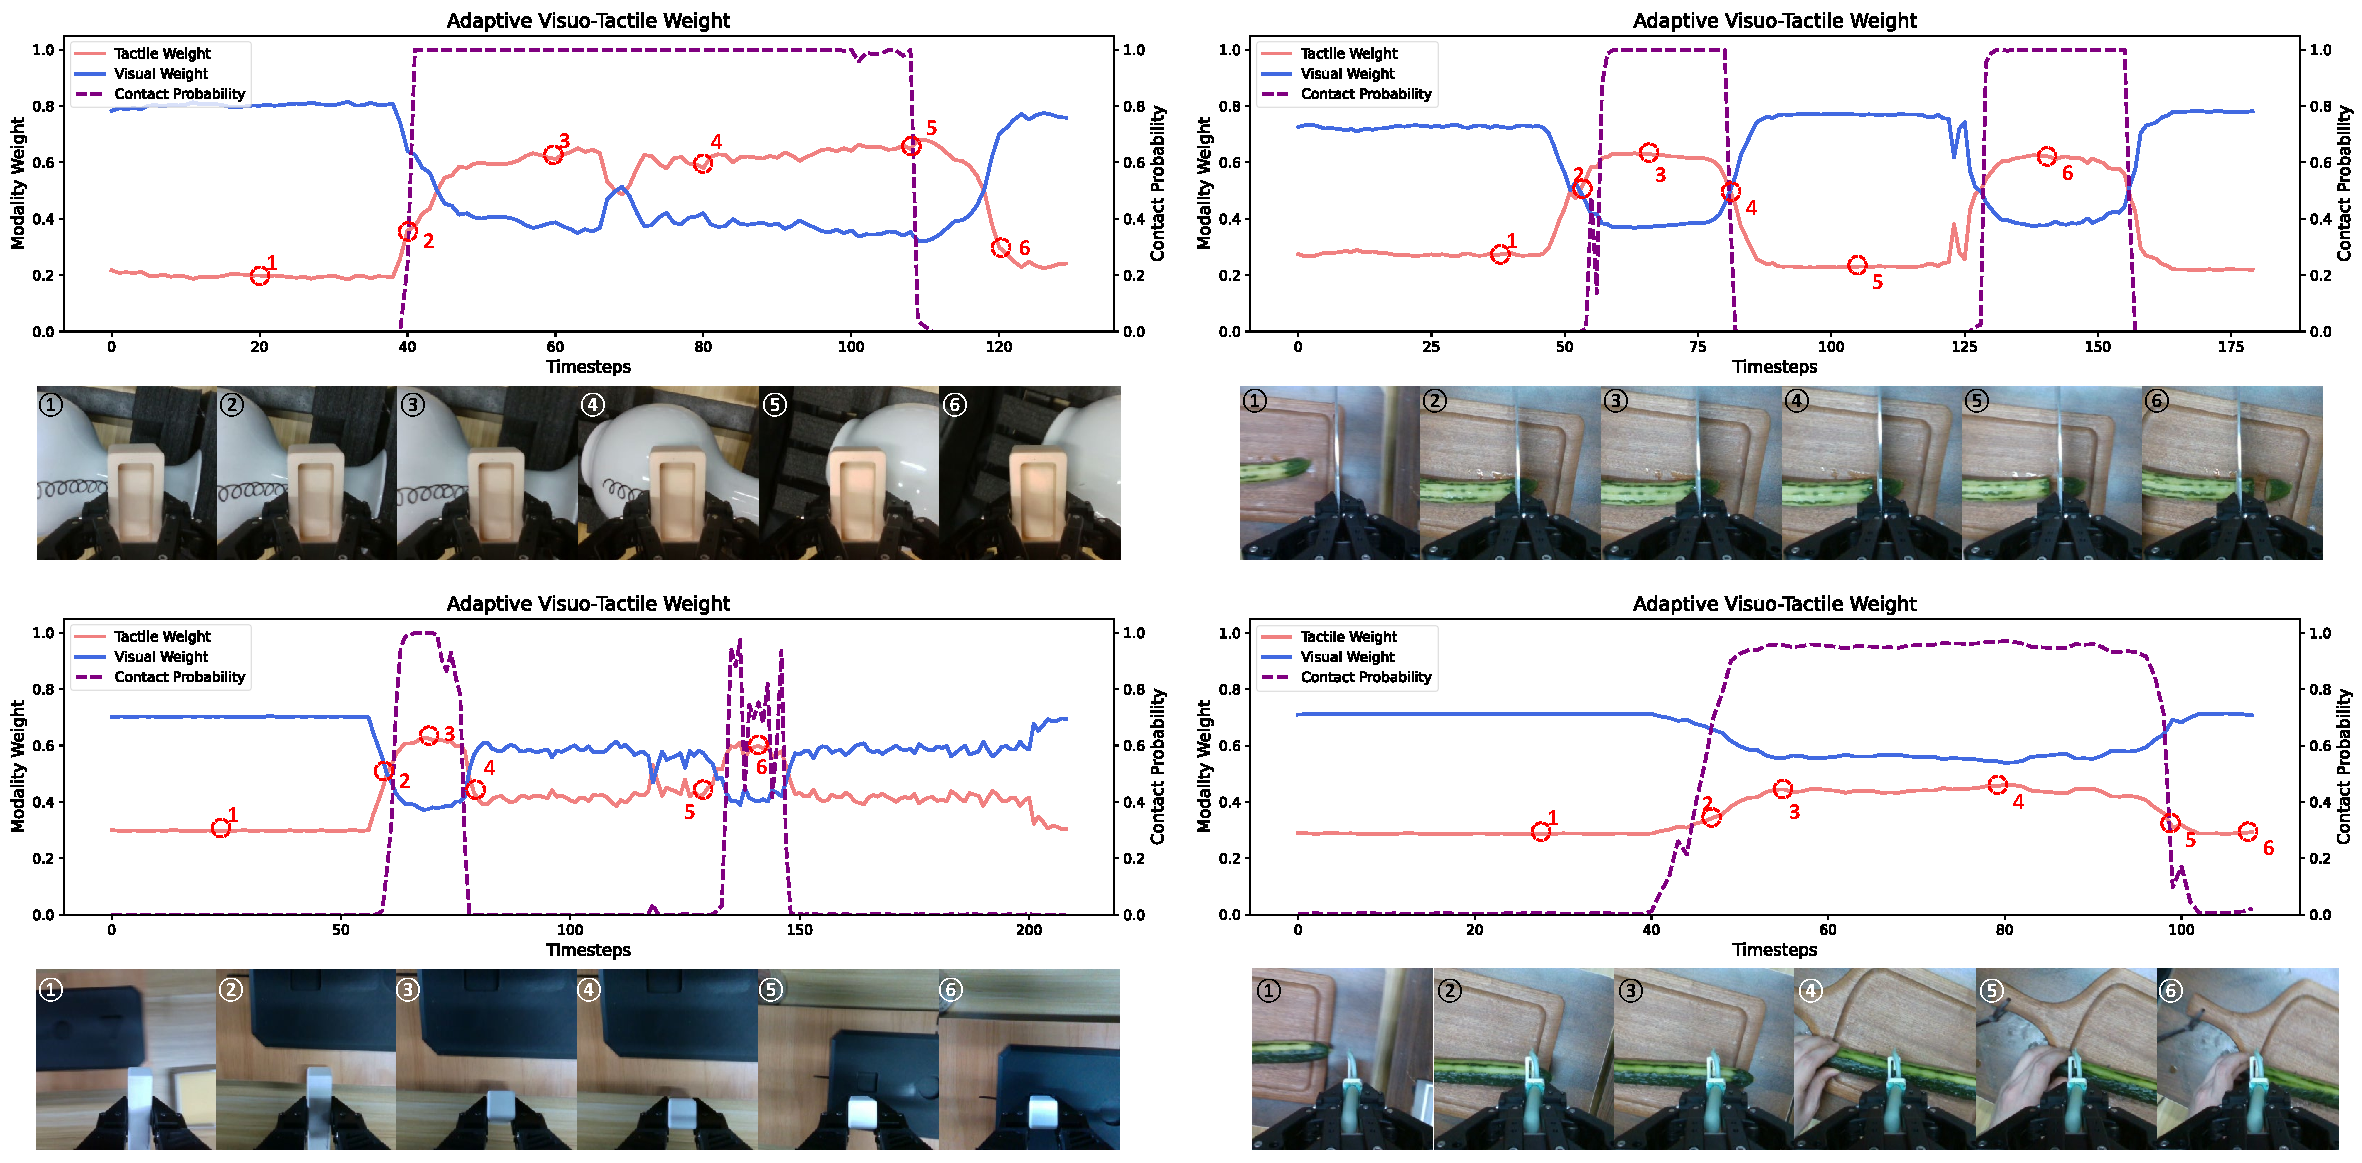
\includegraphics[width=0.95\linewidth]{fig/gate_weight.pdf}
\caption{G\textbf{Gating Fusion Mechanism.} We visualize the temporal evolution of the predicted contact probability (purple), together with the corresponding visual (blue) and tactile (red) weights over the course of task execution.}
\label{fig:gate_weight}
\vspace{-3mm}
\end{figure*}

\begin{figure*}[ht]
\centering
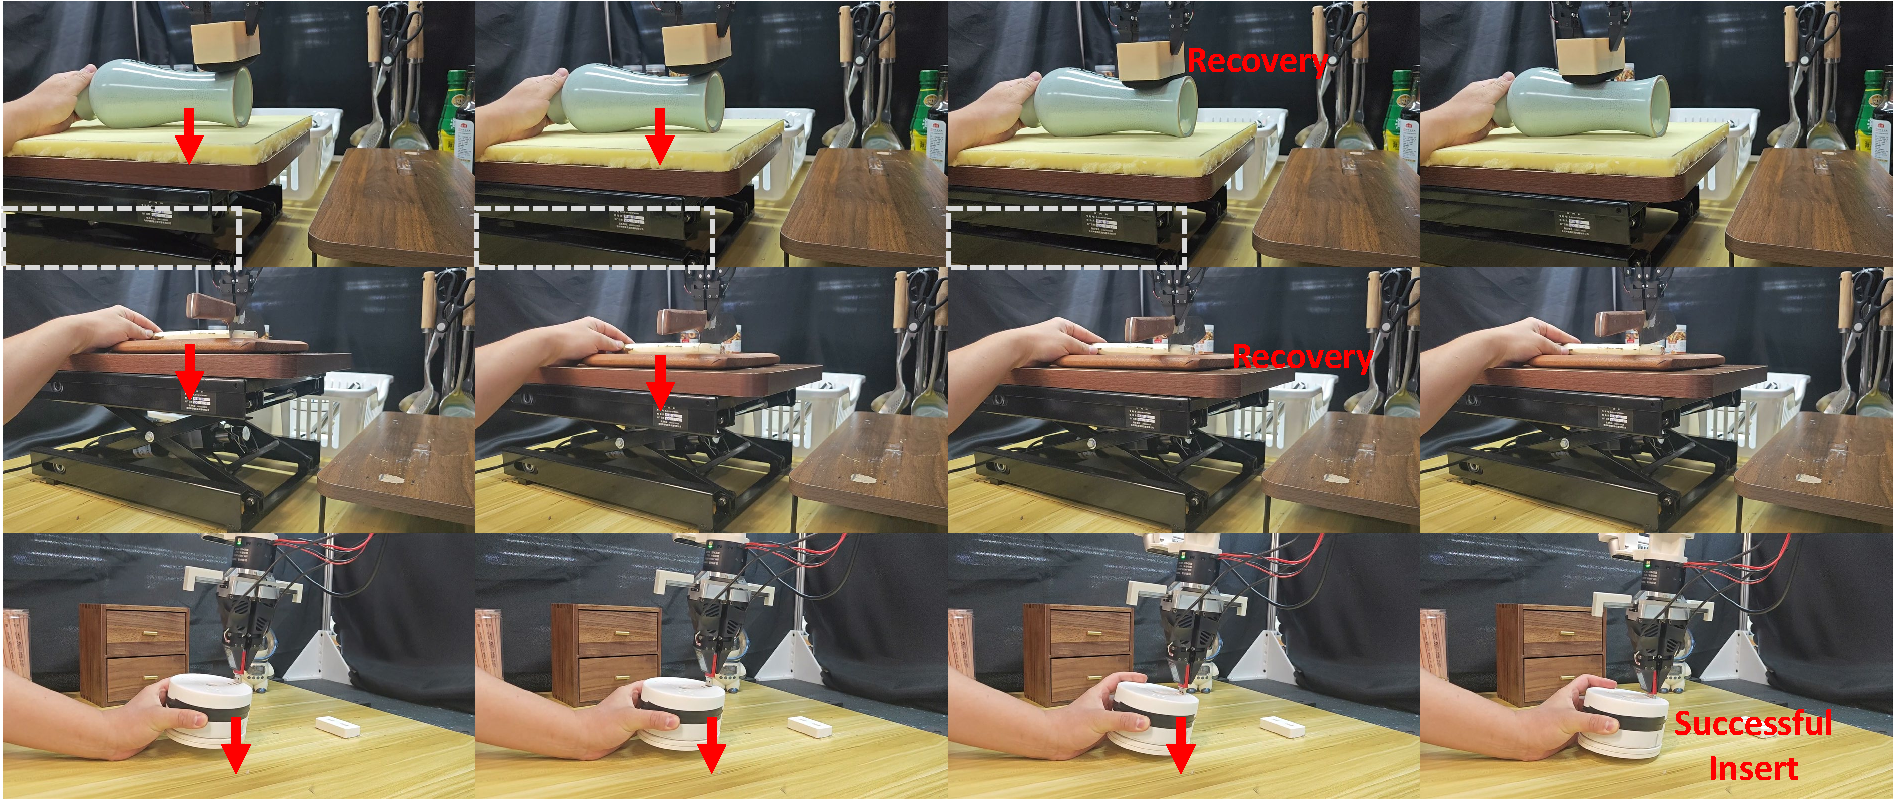
\includegraphics[width=0.95\linewidth]{fig/mp_disturb.pdf}
\caption{\textbf{Perturbation experiments.} We break contact by abruptly lowering the object and demonstrate how the policy rapidly restores contact via the RLTC.}
\label{fig:mp_disturb}
\vspace{-3mm}
\end{figure*}


\noindent \textbf{Necessity of the gating fusion mechanism.}
Next, we evaluate the effectiveness of the gating mechanism for visuo-tactile fusion by comparing two input configurations:
(1) direct concatenation of visual features and LTD-encoded tactile features, and
(2) adaptive fusion using the proposed gating mechanism.
As shown in Table~\ref{tab:ablation_components_scaled}, the gating mechanism improves the average task success rate by approximately 7\% compared to direct concatenation.
We further visualize the predicted contact probability and the modality weights in Fig.~\ref{fig:gate_weight}.
The results show a strong correlation between modality weights and contact states: when no contact occurs, the tactile weight remains close to zero, while it increases significantly as the predicted contact probability rises, indicating that action planning increasingly relies on tactile information during contact.

\noindent \textbf{Effect of tactile prediction.}
To evaluate how policy performance depends on tactile prediction quality, we introduce controlled prediction errors by using world model checkpoints with varying tactile prediction accuracies, corresponding to 80\%, 60\%, 40\%, and 20\% of the performance of the best-performing model.
As shown in Fig.~\ref{fig:prediction}, as prediction accuracy decreases, the policy gradually loses its ability to correctly infer contact states and adjust modality weights, leading to degraded action planning performance. This proves that accurate tactile prediction plays a critical role in our policy.

\begin{figure}[ht]
\centering
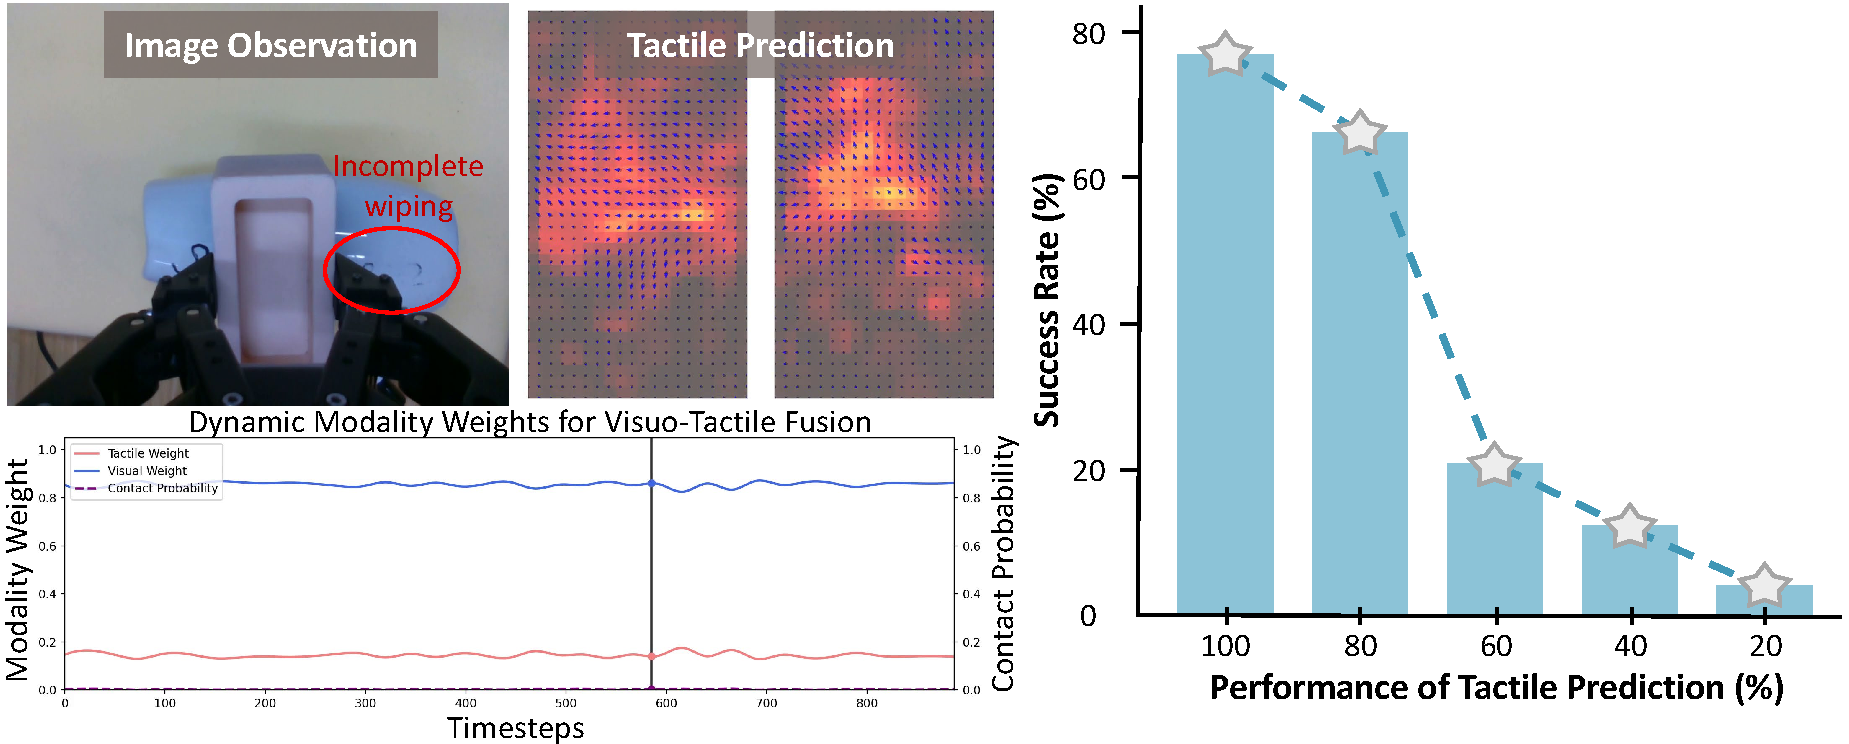
\includegraphics[width=\linewidth]{fig/prediction.pdf}
\caption{\textbf{Effect of tactile prediction accuracy.} \textbf{Left:} At 60\% prediction performance, the model fails to estimate future contact probability, resulting in improper modality weighting. \textbf{Right:} Lower prediction performance leads to a significant drop in success rate.}
\label{fig:prediction}
\vspace{-5mm}
\end{figure}

\noindent \textbf{Effect of generated visual features.}
We also investigate whether incorporating generated visual features improves policy performance.
Experimental results show that adding generated visual features to the policy input does not yield significant performance gains, as shown in Table~\ref{tab:ablation_components_scaled}. Moreover, introducing a visual generation branch significantly reduces inference frequency, as shown in Table~\ref{tab:policy_time}. Therefore, the final policy design relies only on current visual observations rather than on the generation.

\noindent \textbf{Effectiveness of the Reflexive Latent Tactile Controller.}
Finally, we evaluate the contribution of the Reflexive Latent Tactile Controller.
The controller enables high-frequency closed-loop control, allowing the robot to execute actions more stably and improving overall task success rates.
In perturbation experiments, shown in Table~\ref{tab:full_comparison_final_scaled} and Fig.~\ref{fig:mp_disturb}, the controller rapidly responds to environmental perturbations. When perturbations disrupt the current contact state, the high-frequency controller adjusts robot actions to re-establish stable contact.
In tasks requiring strong interaction forces, the controller also adaptively modulates the action magnitude to prevent excessive contact forces.


\section{Conclusion}
In this work, we address two persistent bottlenecks in visuo-tactile manipulation: the scarcity of large-scale, task-diverse training data and the lack of methods that model contact dynamics explicitly while supporting closed-loop tactile control.
On the data side, OmniViTac comprises $21{,}000+$ temporally aligned trajectories spanning $86$ contact-rich tasks organized into six physics-grounded interaction patterns. Systematic analysis of the dataset identifies two structural properties of tactile signals in manipulation, spatial locality, and contact-driven dynamics, which guided the architectural design of OmniVTA.
On the methodology side, OmniVTA integrates self-supervised implicit tactile representation learning, short-horizon visuo-tactile world modeling, contact-aware multimodal fusion, and high-frequency reflexive control within a unified framework. Real-robot experiments across all six interaction categories demonstrate that OmniVTA consistently outperforms existing baselines, with clear advantages in generalization to unseen objects and geometric configurations and robustness to external disturbances.

\section{Acknowledgments}
We want to thank Xiangyu Chen, Yating Feng, Zhijie Yan, Xiang Xiao, Jingxiang Guo, and Yuxing Qin for their efforts in building the OmniViTac dataset.
% \subsection{Limitation and future work}
% This work has several limitations. While OmniViTac provides a comprehensive benchmark for single-arm, gripper-based tactile manipulation, it does not currently encompass the dual-arm setting or other end-effector types, such as dexterous hands. Future work will investigate scaling the world model with larger and more diverse data, extending the framework to dexterous hands and dual-arm manipulation, and exploring cross-embodiment transfer of the visuo-tactile representations.



% \section{Conclusions and Future Work}
% \subsection{Conclusions}
% \subsection{Limitations and Future Works}



\bibliographystyle{elsarticle-num} 
\bibliography{main}{}  


\end{document}